\documentclass[a5paper,english]{ufsc-thesis}
\usepackage[T1]{fontenc}
\usepackage[utf8]{inputenc}
\usepackage{indentfirst}
\usepackage{color}
\usepackage[alf]{abntex2cite}
\usepackage{lastpage}
\usepackage{indentfirst}
\usepackage{color}
\usepackage{graphics}
\usepackage{graphicx}
\usepackage{booktabs}
\usepackage{tabularx}
\usepackage{enumitem}
\usepackage{float}
\usepackage[cache=false]{minted}
\usepackage{pgfplots}
\usepackage{smartdiagram}
\usepackage{tikz}
\usetikzlibrary{shapes,decorations,arrows}
\title{Estudo sobre o uso da linguagem GraphQL na composição de serviços em busca de dados JSON}
\instituicao{Universidade Federal de Santa Catarina}
\centro{Centro Tecnológico -- CTC}
\programa{Curso de Graduação em Sistemas de Informação}
\tipotrabalho{Trabalho de Conclusão de Curso}
\autor{Mateus Maso}
\local{Florianópolis, SC}
\data{\today}
\orientador{Frank Augusto Siqueira}
\preambulo{Trabalho de Conclus\~{a}o de Curso submetido ao Curso de Graduação em Sistemas de Informação para a obtenção do Grau de Bacharel em Sistemas de Informação.}
\assuntos{GraphQL,REST,JSON Hyper-Schema}
\begin{document}
\instituicao[a]{Universidade Federal de Santa Catarina}
\departamento[o]{Departamento de Informática e Estatística}
\curso[o]{Programa de Graduação em Sistemas de Informação}
\documento[o]{{Trabalho de Conclusão de Curso}}
\titulo{Estudo sobre o uso da linguagem GraphQL na composição de dados através de serviços baseados em JSON}
\autor{Mateus Maso}
\grau{Bacharel em Sistemas de Informação}
\local{Florianópolis, SC}
\data{\today}
\orientador{Prof. Dr. Frank Augusto Siqueira}

\capa
\folhaderosto

% \epigrafe{
  Time has told me not to ask for more,
  someday our ocean will find its shore
} {(Nick Drake)}

\paginaepigrafe

\begin{resumo}
  Para acomodar a rápida transformação na demanda por dados em aplicações distribuídas, recentemente tem-se discutido novas maneiras de disponibilizar dados para o consumo eficiente de clientes diversificados. Contudo, as atuais formas de comunicação cliente-servidor têm causado dependência e acoplamento entre o código de busca de dados e a especificação utilizada para acesso da API. Isso porque, para garantir a integridade da comunicação, clientes e serviços precisam estabelecer um contrato de interface de acesso para que não haja mudanças após a implementação do cliente. Para evitar isso, este projeto realiza um estudo sobre o uso da linguagem GraphQL para propor um modelo de comunicação cliente-servidor que não dependa de contrato de API e permita a composição de serviços na busca de dados JSON. Além disso, é desenvolvido uma ferramenta com base no modelo proposto para validar sua aplicabilidade. \\ \\
  \textbf{Palavras-chaves}: GraphQL. REST. JSON Schema.
\end{resumo}
\begin{resumo}[Abstract]
  \begin{otherlanguage*}{english}
  (Arrumar) In order to embrace the growing transformations of flow in which data is access by clients over APIs Web, services that exposes these data had applied efforts in adapt interfaces to  efficient ways to expose data for a diversified consumption of clients. However, the current client implementation approach of the client-server communication model has created dependency and coupling between the client's data fetching code and the API specification used for access. To solve that, this project studies the usage of GraphQL language and API description formats to offer a new cliente-server communication model that avoid coupling due to client fetching code implementation. By automating queries, the model aims to optimize requests, be tolerant of API changes and help fetch data through service composition. Furthermore, a tool is developed based on the proposed model to validate it's aplicability. \\ \\
    \textbf{Key-words}: GraphQL. REST. JSON Hyper-Schema.
  \end{otherlanguage*}
\end{resumo}

\listoffigures
\cleardoublepage
\listoftables*
\cleardoublepage

\begin{siglas}
  \item[AST] Árvore sintática abstrata
  \item[API] Interface de Programação de Aplicação
\end{siglas}
\cleardoublepage

\tableofcontents*
\cleardoublepage

\textual

\chapter{Introdução}

Neste capítulo é apresentado o atual cenário do mercado de APIs Web, o problema de acoplamento encontrado na forma de comunicação cliente-servidor para busca de dados e a proposta do projeto de uma ferramenta para solucionar este problema de acoplamento, além dos objetivos e metodologia de pesquisa utilizados em seu desenvolvimento.

\section[Descrição do Problema]{Descrição do Problema}

Em 2005, ocorreu uma grande transição no modelo de comunicação entre aplicações distribuídas, onde estas passaram a utilizar amplamente o protocolo HTTP e o modelo cliente-servidor para a troca de informações na World Wide Web. Um dos principais motivos que contribuiu na época para esta crescente transição, segundo Duvander, foi devido a facilidade de aplicações em expor sua API através do estilo de arquitetura REST, assim como clientes em se comunicar com essas APIs. \cite{Duvander2013-2}

Hoje, empresas como Facebook e Netflix mostram que, independente do estilo de arquitetura, construir APIs Web é, não apenas essencial para entrar rápido no mercado de plataformas emergentes, como também um novo meio de agregar valor em seu próprio modelo de negócio e oferecer uma melhor experiência a seus usuários. \cite{Art2016}

Contudo, após anos de sua popularização e diversas implementações em clientes com base em seu modelo de comunicação, serviços têm mostrado dificuldades em realizar mudanças em suas APIs sem comprometer a comunicação. Isso porque clientes estão implementando em seu código de busca chamadas de forma direta à especificação de APIs Web, ocasionando um acoplamento muitas vezes indesejado pelos serviços.

Além disso, este acoplamento tem dificultado a adoção de novas tecnologias e estilos de arquitetura por serviços. que necessitam de alterações na especificação da API, pois não conseguem convencer seus benefícios em troca da custosa transição e reimplementação no seu código de busca que clientes vão precisar passar.

\section[Objetivos]{Objetivos}

Com o objetivo de resolver o problema de acoplamento mencionado anteriormente, este trabalho propõe um novo modelo de comunicação cliente-servidor através da automação na execução de consultas de dados sobre APIs Web. Dessa forma, o modelo visa direcionar desenvolvedores de clientes à implementação de códigos de busca independente de especificação de API. Resultando no desenvolvimento de clientes tolerante à mudanças na especificação.

Além disso, o modelo proposto prevê o desenvolvimento de uma ferramenta para servir como intermediador na comunicação e realizar a automação de consultas. Permitindo também a implementação de otimizações de requisição e a composição de serviços para busca de dados. \\

\textbf{Objetivos específicos} \\

No intuito de atingir o objetivo geral do trabalho, serão buscados os seguintes objetivos específicos:

\begin{itemize}
\item Propor modelo de comunicação replicável e agnóstico à plataforma.
\item Desenvolver ferramenta prevista pelo modelo para plataforma Web.
\item Validar a ferramenta na comunicação entre clientes e APIs Web.
\item Promover a busca de dados através de linguagens de consulta.
\item Promover a documentação de APIs através de formatos de descrição. \\
\end{itemize}

\textbf{Limites da pesquisa} \\

O escopo do presente trabalho é delimitado da seguinte forma:

\begin{itemize}
\item Enfase na comunicação entre clientes e APIs REST.
\item Enfase na tecnologia GraphQL para linguagem de consulta.
\item Enfase na tecnologia JSON Hyper-Schema para descrição de APIs.
\item Testes de composição de serviços não aplicados para a ferramenta.
\end{itemize}

\section[Metodologia]{Metodologia}

A primeira etapa do trabalho foi a idealização do modelo, onde foi levantada uma série de perguntas que culminaram em um profundo estudo para comprovar se era possível resolver o problema e de que forma a solução seria implementada. Adicionalmente, foram identificadas as tecnologias que poderiam ser usadas para ajudar no desenvolvimento da ferramenta proposta pelo modelo e facilitar sua replicação em diversas plataformas.

Em seguida, foi pensado na criação de uma interface para a ferramenta que fosse simples de usar, rodasse em serviços GraphQL já existentes e pudesse ser integrado em APIs REST que já possuem algum formato de descrição de metadados.

Após isso, foi realizado um PoC\footnote{
  Proof of concept ou Prova de conceito
} para validar o protótipo do modelo. Em paralelo, iniciou-se o processo de escrita da monografia, implementação da ferramenta e preparação de um ambiente de validação que pudesse enfatizar bem os problemas reais que clientes Web têm presenciado devido a este acoplamento na busca de dados. 

Por fim, com o objetivo de apresentar uma comprovação da tese, foram postos para rodar os testes de validação, coletando os dados e apresentando os resultados analisados ao lado de ilustrações com gráficos.
\section[Organização do Texto]{Organização do Texto}

O texto está organizado em 6 capítulos. O primeiro aborda os conceitos de fundamentos utilizados para entender o modelo, a implementação da ferramenta e o ambiente de validação. Em seguida, em um capítulo à parte, é descrita a tecnologia GraphQL, responsável por possibilitar a realização do trabalho. Após, é especificado todo o processo de desenvolvimento do trabalho como o planejamento de projeto e implementação. Seguido pelo capítulo de validação, onde é preparado o ambiente testes, executados e analisados através de gráficos. Por fim, no último capítulo, é exposto a conclusão sobre o trabalho, além de propor melhorias a serem desenvolvidas para trabalhos futuros.


\chapter{Fundamentos}

Neste capítulo são estabelecidos os principais conceitos utilizados ao longo do trabalho. Será conduzido uma breve abordagem sobre os fundamentos de serialização de dados; seguido pelo formato de representação JSON; o estilo de arquitetura baseado em recursos e formas para descrição de seus metadados.

\section[Serialização de Dados]{Serialização de Dados}

Na ciência da computação, serialização de dados é um processo de tradução usado para converter estruturas de dados\footnote{
  Uma estrutura de dados é uma forma abstrata de representar e organizar dados. Seu objetivo é ajudar a reduzir complexidade, podendo armazenar dados de diferentes tipos, como números, strings ou até mesmo outras estruturas de dados.
} em formatos que possam ser armazenados, transmitidos e reconstruídos por um mesmo ou por outro ambiente computacional. \cite{Cline2016}

Dados serializados normalmente têm um tempo de vida maior que suas aplicações de origem e, ao serem armazenados em disco ou transmitidos pela rede, possuem representação diferente do que sua estrutura em memória. Para se ler dados serializados em memória é preciso realizar o processo inverso, também chamado de desserialização, onde estes passam a ser representados por estruturas da linguagem de execução. \cite{Guller2016}
  
\begin{figure}[H]
  \centering
  \smartdiagramset{circular distance=2cm,uniform arrow color=true,arrow line width=1pt,arrow color=gray!50!black,uniform color list=white for 6 items,font=\small,text width=2.0cm,module minimum width=2.0cm,module minimum height=1.5cm,arrow tip=to}
  \smartdiagram[flow diagram:horizontal]{Estrutura de dados,Serialização,Estrutura serializada,Desserialização}
  \caption{Processo de serialização e desserialização}
\end{figure}

Este processo, embora demande tempo, permitiu que aplicações fizessem o consumo de informações de forma distribuída, contribuindo com o aumento do volume de dados que circulam pela internet. Além disso, fez-se necessária a seleção adequada de formatos de serialização cuja estrutura não prejudicasse o desempenho de aplicações na busca por dados. \cite{SumarayMakki2012}

Segundo a Cisco Systems, de 2014 para 2015, houve um aumento de 21\% no volume de tráfego de dados registrados apenas por seus aparelhos. As categoria Web, Email e Data foram responsáveis por representar aproximadamente 7,558 petabytes de dados transmitidos por seus clientes durante um mês. \cite{Cisco2016}

Para suprir esta alta demanda, diversos formatos de serialização foram introduzidos para melhor atender os problemas de desempenho experienciados por serviços. Dentre eles, tempo de serialização e desserialização, tamanho de transferência, flexibilidade de uso, facilidade de leitura, automação, suporte para linguagem, entre outros. \cite{Guller2016}

\begin{table}[ht!]
  \centering
  \resizebox{\columnwidth}{!}{
    \begin{tabular}{|c|c|c|c|c|}
      \hline
      Formato & Especificação & Codificação & Legibilidade & Esquema/IDL \\
      \hline
      XML & Padronizada & Textual & Sim & Sim \\
      \hline
      JSON & Padronizada & Textual & Sim & Parcial \\
      \hline
      YAML & Padronizada & Textual & Sim & Parcial \\
      \hline
      Avro & Padronizada & Binário & Não & Sim \\
      \hline
      P. Buffers & Padronizada & Binário & Parcial & Sim \\
      \hline
      Thrift & Não Padronizada & Binário & Parcial & Sim \\
      \hline
    \end{tabular}
  }
  \caption{Comparação de formatos de serialização}
\end{table}

Para melhor entender cada formato, será feita uma abordagem sobre algumas das categorias de classificação utilizadas para estudar o desempenho dos formatos existentes hoje em dia. \\

\textbf{Especificação} \\

Um formato pode ter sua especificação classificada como padronizada ou não padronizada. Uma especificação padronizada é regida por requisitos que auxiliam na reprodutibilidade do processo em outras linguagens para maximização da compatibilidade e minimização de erros. Ao contrário, dada uma linguagem de programação, não é garantido que sua implementação esteja seguindo os padrões e poderá ser considerado como não padronizada. \cite{McDermid1991} \\

\textbf{Codificação} \\

Codificação é o processo de sequenciamento de caracteres usado na representação dos dados transmitidos ou armazenados. É possível classificar em dois tipos: textuais e binários. Formatos baseados em texto podem ser lidos diretamente através de editores de texto. Já um formato binário faz o uso intensivo da codificação e decodificação para salvar espaço. \cite{Queiros2014} \\

\textbf{Legibilidade} \\

Ao representar estruturas de dados em formatos de serialização para que máquinas possam fazer a leitura, não é garantido, no entanto, que esta representação também seja legível por seres humanos.

Para que um formato seja legível por humanos (\textit{human-readable}), além de máquinas, pessoas devem conseguir ler e dizer o que está sendo representado na estrutura, mesmo fora de contexto. Para desenvolvedores, este detalhe é essencial no processo de debugging\footnote{
  Depuração é o processo de encontrar e reduzir defeitos num aplicativo de software ou mesmo em hardware.
}. Nota-se que a leitura de um formato é diferente de seu entendimento, uma vez que nem todos os formatos possuem maneiras de descrever seus metadados. O formato JSON, por exemplo, é baseado em texto e tem como objetivo a facilidade de uso e legibilidade por desenvolvedores. Nem sempre, contudo, é possível identificar o que está sendo representado em suas estruturas. \cite{SumarayMakki2012} \\

\textbf{Esquema/IDL} \\

Com objetivo de entender o que está sendo representado, alguns formatos disponibilizam na sua especificação maneiras de descrever metadados. Esta categoria é importante principalmente para que máquinas consigam inferir quais estruturas estão sendo lidas e, assim, tomar decisões de forma autônoma.

Um formato descritivo normalmente disponibiliza estruturas como esquemas IDL\footnote{
  Linguagem de descrição utilizada para descrever a interface dos componentes de um software.
} para descrição da própria representação. À medida que estas descrições são incorporadas dentro da mesma representação, é possível classificar estes formatos como sendo auto-descritivos. \cite{Rentachintala2014}

\section{JSON}

JSON ou Javascript Object Notation é um formato de serialização de dados human-readable baseado em texto com especificação padronizada e parcialmente descritivo. Foi desenvolvido por Douglas Crockford com o objetivo de representar dados em uma maneira simples, leve e flexível através da redução na sobrecarga de marcações comparado ao formato XML.

Por ter se adaptado bem no ambiente de aplicações distribuídas, este formato acabou sendo amplamente utilizado em serviços como principal forma de representação de dados serializados. \cite{Duvander2013}

Na sua essência, o JSON foi construído com base em quatro tipos primitivos de dados e outros dois para composição. Cada tipo possui seu respectivo correspondente na maioria das linguagens de programação, embora possam ser identificados por nomes diferentes. \cite{Droettboom2015}

\begin{table}[H]
  \centering
  \begin{tabular}{|c|c|c|c|c|}
    \hline
    Tipo & Exemplo de Valor \\
    \hline
    object & \mintinline[fontsize=\footnotesize]{text}{ {"chave1": "valor1", "chave2": "valor2"} } \\
    \hline
    array & \mintinline[fontsize=\footnotesize]{text}{ ["primeiro", "segundo", "terceiro"] } \\
    \hline
    number & \mintinline[fontsize=\footnotesize]{text}{ 1, -1, 2.9999 } \\
    \hline
    string & \mintinline[fontsize=\footnotesize]{text}{ "Isso é uma string" } \\
    \hline
    boolean & \mintinline[fontsize=\footnotesize]{text}{ true, false } \\
    \hline
    null & \mintinline[fontsize=\footnotesize]{text}{ null } \\
    \hline
  \end{tabular}
  \caption{Tipos de valores em JSON}
\end{table}

Através da composição de listas, objetos e tipos primitivos, consegue-se representar complexas estruturas de dados. Não existe, no entanto, um único padrão de representação. Dada uma estrutura, é possível representá-la de inúmeras maneiras. A seguir estão duas formas diferentes de representação em JSON de uma entidade “pessoa”:
 \cite{Droettboom2015}

\begin{figure}[H]
  \centering
  \begin{minted}[frame=single,framesep=10pt,fontsize=\footnotesize]{text}
    {
      "nome": "Mateus Maso",
      "aniversario": "25 de março de 1992",
      "cidade": "Florianópolis, SC, Brasil"
    }
  \end{minted}
  \caption{Primeiro exemplo de representação JSON}
\end{figure}

\begin{figure}[H]
  \centering
  \begin{minted}[frame=single,framesep=10pt,fontsize=\footnotesize]{text}
    {
      "nome": "Mateus",
      "sobrenome": "Maso",
      "nascimento": "25-03-1992",
      "cidade": {
        "nome": "Florianópolis",
        "estado": "SC",
        "pais": "Brasil"
      }
    }
  \end{minted}
  \caption{Segundo exemplo de representação JSON}
\end{figure}

Ambas representações são válidas, apesar da figura 4 estar representando os dados em uma estrutura um pouco mais formal. No entanto, por ser um formato não descritivo, a responsabilidade de entender o que está sendo representado vai depender da análise crítica ou conhecimento prévio dos desenvolvedores. Já uma máquina, sem conhecer o contexto, não saberia como interpretar os dados de forma correta. \cite{Droettboom2015}

Para resolver isso, será abordado em seguida um dos formatos existentes hoje em dia para a descrição de estruturas JSON.

\section[JSON Schema]{JSON Schema}

JSON Schema é uma linguagem de definição projetada para descrever estruturas de dados JSON por meio de esquemas. Proposta em 2009 por Kris Zyp, teve como objetivo fornecer um contrato para que aplicações soubessem como trabalhar e interagir com estruturas de dados. Por meio deste, é possível prever representações e assim realizar operações de validação, documentação, navegação por \textit{hyperlinks} e controle de iteração. \cite{Zyp2013}

Por ser uma linguagem de simples uso, para modelar um esquema basta construir um objeto JSON utilizando um subconjunto válido de chaves especias descritas pela linguagem. No entanto, funcionalidades como descrição de estruturas multimídia\footnote{
 Capaz de reunir diversas mídias, como imagens, textos, vídeos e audio digital, por exemplo.
} e a navegação de dados são apenas disponibilizadas no formato JSON Hyper-Schema, uma variação da linguagem de especificação. \cite{Jackson2016}

\begin{figure}[H]
  \centering
  \begin{minted}[frame=single,framesep=10pt,fontsize=\footnotesize]{text}
    {
      "\$schema": "http://json-schema.org/draft-04/schema#",
      "title": "Pessoa",
      "description": "Uma pessoa",
      "type": "object",
      "required": ["nome", "aniversario"],
      "properties": {
        "nome": {
          "type": "string"
        },
        "aniversario": {
          "type": "string"
        },
        "cidade": {
          "type": "string"
        }
      }
    }
  \end{minted}
  \caption{JSON Schema para Figura 3}
\end{figure}

\begin{figure}[H]
  \centering
  \begin{minted}[frame=single,framesep=10pt,fontsize=\footnotesize]{text}
    {
      "\$schema": "http://json-schema.org/draft-04/hyper-schema#",
      ...,
      "properties": {
        ...,
        "foto": {
          "media": {
            "binaryEncoding": "base64",
            "type": "image/png"
          }
        }
      },
      "links": [
        {
          "rel": "foto",
          "href": "/{id}.png",
          "mediaType": "image/png"
        }
      ]
    }
  \end{minted}
  \caption{JSON Hyper-Schema para Figura 3}
\end{figure}

Ao exemplo das figuras 4 e 5, ambos os esquemas asseguram que, dada uma estrutura JSON, para que esta seja reconhecida como uma entidade “pessoa”, deve conter as propriedades "nome" e "aniversario" com valores do tipo "string". Já na figura 5, além das estruturas definidas pela figura 4, é descrita uma nova propriedade "foto" do tipo multimídia, além de como navegar em busca desta informação.

Em casos onde a complexidade de um esquema começa a crescer, é comum a definição de sub-esquemas através da chave “definitions”. Desta forma, podem ser referenciadas pela chave "\$ref" permitindo o reuso de estruturas dentro de um esquema. Vale lembrar que a chave “definitions” é apenas um mecanismo útil para definir esquemas em um lugar comum, entretanto, não sugerem que estas propriedades sejam validadas em um objeto ao menos que referenciadas em outras estruturas do esquema. \cite{Leach2014}

\begin{figure}[H]
  \centering
  \begin{minted}[frame=single,framesep=10pt,fontsize=\footnotesize]{text}
    {
      "\$schema": "http://json-schema.org/draft-04/hyper-schema#",
      ...,
      "definitions": {
        "cidade": {
          "type": "string",
          "properties": {
            "nome": { "type": "string" },
            "estado": { "type": "string" },
            "pais": { "type": "string" }
          }
        }
      },
      "properties": {
        ...,
        "cidade": {
          "\$ref": "#/definitions/cidade"
        }
      },
      "links": [
        ...,
        {
          "rel": "cidade",
          "href": "/{id}/cidade",
          "targetSchema": {
            "\$ref": "#/definitions/cidade"
          }
        }
      ]
    }
  \end{minted}
  \caption{JSON Hyper-Schema para Figura 4 usando \$ref}
\end{figure}

Como boa prática, é recomendado (mas não necessário) o uso da chave especial “\$schema” para determinar quando uma estrutura JSON está sendo representada em forma de esquema. Na tabela 3 são descritas algumas das chaves especiais usadas para descrever objetos em esquemas. \cite{Droettboom2015}

\begin{table}[ht!]
  \centering
  \begin{tabular}{|c|c|}
    \hline
    Chave & Descrição \\
    \hline
    \$schema & Identificador de versão \\
    \hline
    type & Tipo de dado \\
    \hline
    title & Nome da estrutura \\
    \hline
    description & Propósito da estrutura \\
    \hline
    required & Lista de propriedades com presença obrigatória \\
    \hline
    properties & Propriedades usadas para validar uma estrutura \\
    \hline
    definitions & Propriedades (sub-esquemas) para referência \\
    \hline
    ... & ... \\
    \hline
    links & Lista de Link Description Objects (LDO) \\
    \hline
  \end{tabular}
  \caption{Subconjunto de chaves especiais JSON Schema}
\end{table}

De certa forma, JSON Schema continua sendo uma das únicas tentativas sérias de propor uma linguagem de definição para o formato JSON. Contudo, ainda está longe de ser considerada padrão, mas já há um número crescente de aplicações que suportam o formato, além de uma quantidade significativa de ferramentas que permitem sua validação. \cite{PezoaEtAl2016}

Vale lembrar também que, segundo Leach, com o recente surgimento de grandes formatos de descrição de APIs ao longo dos últimos anos, JSON Hyper-Schema tem-se tornado uma ótima opção para descrever a navegação para acesso de interfaces, como por exemplo nome de método, estruturas de chamada e resposta, entre outros relacionamentos. \cite{Leach2014}

Nas próximas seções será abordado um dos estilos de arquitetura mais utilizados hoje em dia em APIs Web, além de soluções encontradas no mercado para descrição deste tipo de API em serviços.

\section{REST}

REST (\textit{Representational State Transfer}) é um estilo de arquitetura usada para a comunicação de sistemas distribuídos através do protocolo HTTP. Foi introduzido por Roy Fielding em 2000 com o objetivo de oferecer às aplicações web um modelo de interface de acesso baseada em recursos. Além disso, descreve seis tipos de restrições que serviços deveriam aplicar para ganho de performance, escalabilidade, simplicidade, modificabilidade, visibilidade, portabilidade e confiabilidade.

Em virtude de causar grande repercussão após sua publicação, o termo REST, segundo Richardson, acabou sofrendo diversas interpretações durante o tempo e sua descrição foi representada de formas não originalmente propostas por Fielding \cite{RichardsonEtAl2013}. Alguns descrevem que serviços que violam essas restrições não podem ser considerados RESTful. Para Wildermuth, apesar de reconhecer as vantagens de cada restrição, serviços web devem usá-los de forma pragmática \cite{Wildermuth2015}.

Ao ser introduzido no mercado de APIs, REST acabou se adaptando bem por ter se mostrado uma solução de fácil acesso em clientes web, dispositivos móveis e de IoT\footnote{
  Do inglês \textit{Internet of Things} (Intenet das Coisas).
}. Segundo Pautasso, a eliminação da complexidade existente em Web Services antes de sua publicação em 2000 fez com que REST fosse considerado um dos principais responsáveis pela popularização de arquiteturas orientada a serviços. \cite{PautassoEtAl2008}

\begin{figure}[H]
  \centering    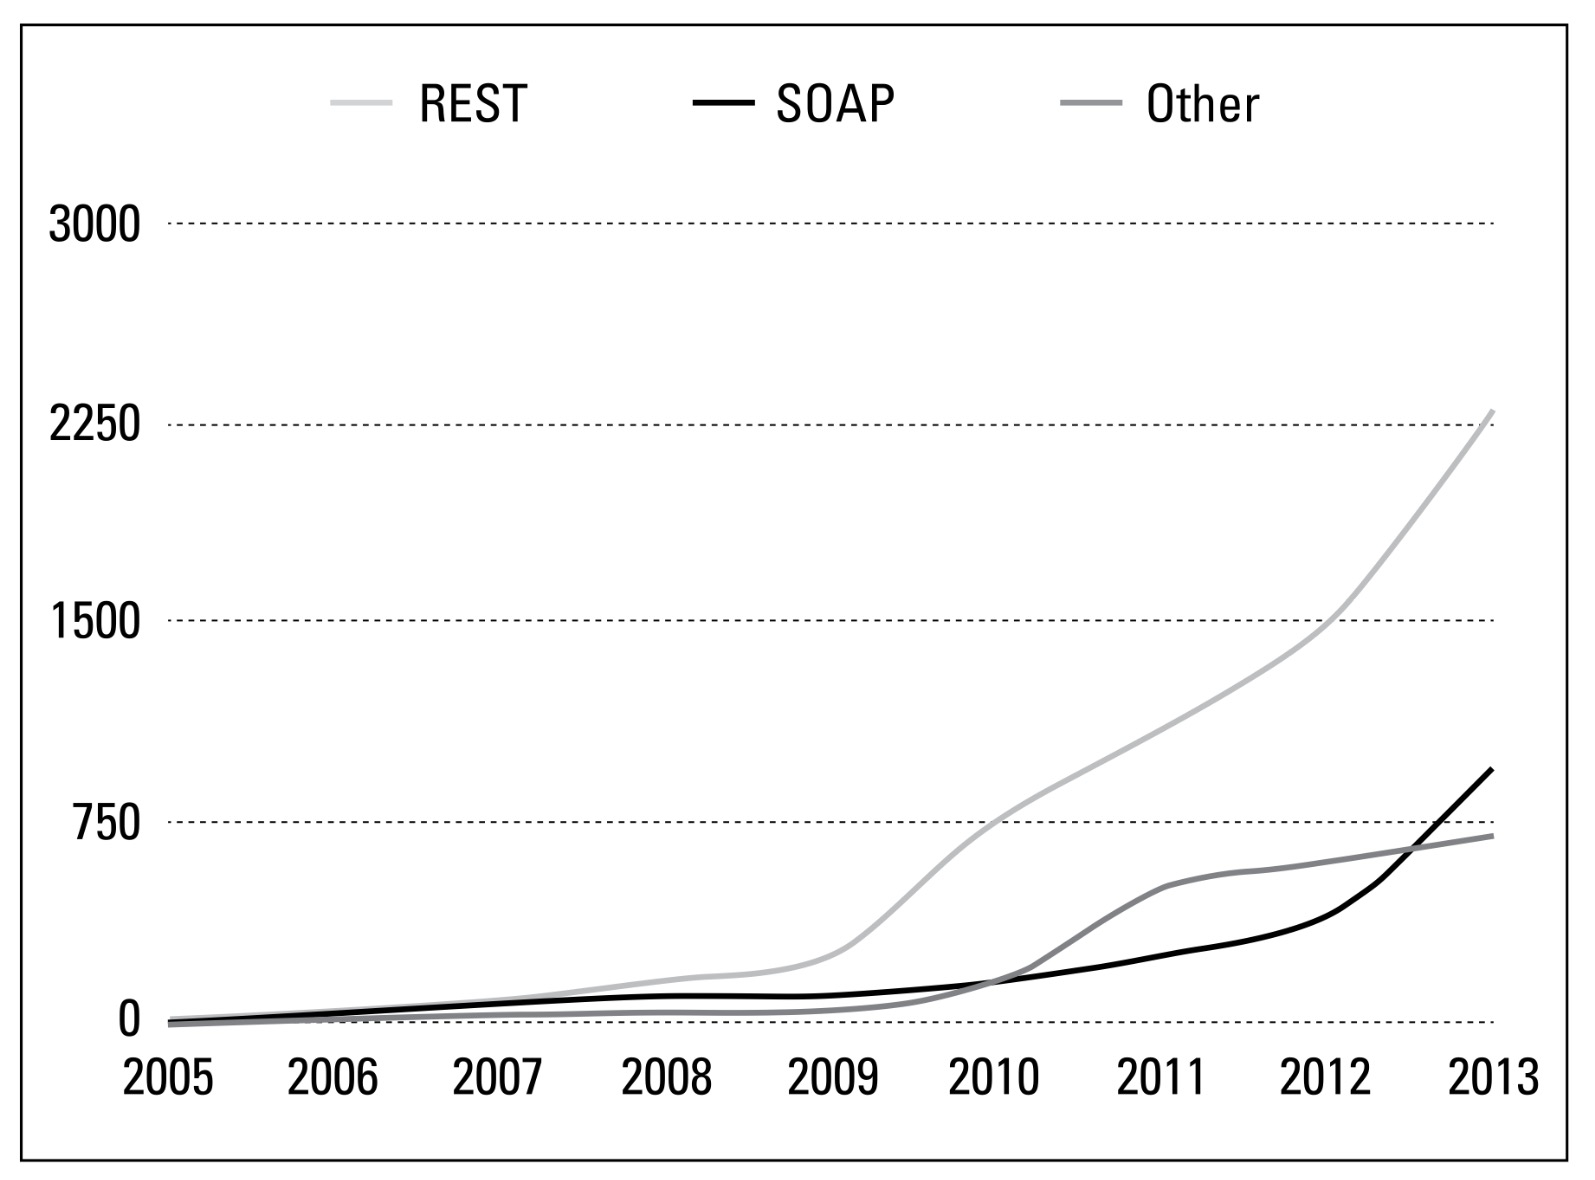
\includegraphics[width=0.9\textwidth,height=\textheight,keepaspectratio]{figuras/api-styles.jpg}
  \caption{Distribuição de estilos e protocolos para APIs}
\end{figure}
% CITAR A FIGURA NO TEXTO

A seguir será apresentada uma visão geral sobre as restrições propostas por Fielding para a implementação em arquiteturas web, além de ser examinado o impacto de cada restrição nesses sistemas distribuídos. \\

\textbf{Cliente-Servidor} \\

Nesta primeira restrição, não existe conexão entre cliente e servidor, mas sim a espera do servidor por pedidos de clientes através de chamada e resposta. O cliente (consumidor do serviço) não se preocupa com tarefas de comunicação de banco de dados, gerenciamento de cache, entre outros. O mesmo ocorre como o servidor (prestador de serviços), que não está preocupado com as tarefas do cliente como interface ou experiência do usuário, por exemplo. Isso permite a evolução independente dos dois ambientes, desde que a interface usada para comunicação entre o cliente e o servidor não seja alterada. \cite{Fielding2000} \\

\textbf{Sem Estado} \\

Esta restrição ajuda na viabilidade, confiabilidade e escalabilidade de sistemas distribuídos, pois garante que chamadas à API não estejam vinculadas a um determinado servidor. Como HTTP é um protocolo sem conexão, cada requisição deve conter todas as informações necessárias para que um servidor entenda o que um cliente está executando. Para Wildermuth, no entanto, dependendo da diversidade no número de clientes, ao manter um servidor sem estado, perder-se o controle no tamanho da estrutura de resposta necessária para atender a demanda de todos os clientes. \cite{Wildermuth2015} \\

\textbf{Interface Uniforme} \\

Em essência, Fielding propõe que aplicações façam o uso de verbos HTTP (POST, GET, PUT, DELETE) e identificadores uniformes de recursos (URIs) para mapear operações em ambientes distribuídos e minimizar o acoplamento entre cliente-servidor. Essas regras de acesso são: \cite{Fielding2000}

\begin{itemize}[noitemsep]
\item Identificação de Recursos: Cada recurso deve ser disponibilizado através de uma URI específica e coesa. (Exemplo: GET /customers/1)
\item Manipulação de Recursos através de Representações: Um recurso pode ser representado em diferentes formatos para diferentes clientes. (Exemplo: HTML, XML, JSON)
\item Resposta Auto-explicativa: Metadados devem ser adicionados na requisição e resposta de um recurso para descrever seu estado atual ou desejado. (Exemplo: código de resposta HTTP, Host, Content-Type)
\item HATEOAS (
 \textit{Hypermedia as the Engine of Application State}): Caso um recurso possua relacionamentos, ao ser representado, estes devem estar especificados em forma de \textit{hyperlinks} para facilitar a navegação de dados por clientes.
\end{itemize}

\textbf{Separação em Camadas} \\

Um dos princípios desta restrição está em evitar que clientes façam diretamente requisição para o servidor sem antes passar por um intermediário, como por exemplo um balanceador de caga (\textit{load balancer})\footnote{
  Técnica para distribuir a carga de trabalho uniformemente entre dois ou mais computadores
}. Desse modo, fica assegurado que clientes apenas se preocupem com a comunicação, deixando que intermediários lidem com a distribuição de requisições. \cite{Fielding2000} \\

\textbf{Código sob Demanda} \\

Apesar de ser a única restrição opcional do estilo, ela permite que servidores disponibilizem código em forma de script para que seja executado no cliente. Dessa forma, a lógica de serviço do servidor é estendida para seus clientes. \cite{Fielding2000} \\

\textbf{Cache} \\

Visa aumentar o desempenho de um serviço. Quando um recurso é acessado por mais de um cliente, se não houve mudança é recomendado que a resposta seja armazenada em cache, evitando o processamento desnecessário. Isso significa que servidores, quando possível, devem implementar regras de cache para beneficio de ambos os ambientes. \cite{Fielding2000}

\section[Descrição de API REST]{Descrição de API REST}

Atualmente, o processo de descrição de APIs tem-se tornado um dos principais fatores de sucesso na aceitação de serviços por desenvolvedores. No entanto, diferente do processo de implementação, a prática de descrição de APIs REST ainda continua sendo feita em sua maior parte manualmente através de linguagem natural. Isso porque REST não apresenta uma forma de documentação externa para descrição de pontos de acesso. \cite{LuckyEtAl2016}

Ao invés, Fielding propõe a descrição dinâmica de APIs através do uso de hiperlinks na representação de recursos para navegação de dados (HATEOAS). Contudo, para Knupp, a solução proposta por Fielding é questionável, pois na sua visão dificulta a legibilidade da interface de acesso, não prevê documentação, cria complexidade de implementação e aumenta de forma significativa o tamanho de resposta. \cite{Knupp2016}

Em busca de oferecer uma solução simples e completa para descrição de APIs REST, foram introduzidas nos últimos anos diversas soluções por empresas e comunidades de desenvolvimento. A seguir, são descritas três das linguagens e formatos que maior ganharam popularidade devido a sua facilidade de uso e legibilidade por humanos e máquinas. \cite{Sandoval2015}

\begin{description}[leftmargin=8em,style=nextline]
  \item[\textbf{OpenAPI}] 
    \begin{enumerate}
        \item[\textbf{+}] Amplamente adotada, ampla comunidade, suporte à diversas linguagens.
        \item[\textbf{$-$}] Carece de especificações avançadas de metadados.
    \end{enumerate}
  \item[\textbf{RAML}] 
    \begin{enumerate}
      \item[\textbf{+}] Suporte à especificação avançada de metadados, adoção significativa, formato legível, suporte da indústria.
       \item[\textbf{$-$}] Falta de ferramentas de auxílio, não comprovada à longo prazo.
    \end{enumerate}
  \item[\textbf{API Blueprint}] 
    \begin{enumerate}
      \item[\textbf{+}] Fácil de entender e simples de escrever.
       \item[\textbf{$-$}] Pouca adoção, carece de especificações avançadas de metadados, difícil de executar.
    \end{enumerate}
\end{description}

Como ainda não existe uma padronização de formato (externo) para descrição de APIs, novas tecnologias estão sujeitas à surgir para melhor se adaptar a comunidade de desenvolvimento. Uma delas, não mencionada anteriormente é o JSON Hyper-Schema que, recentemente através de Lynn e Leach, mostrou ser um método simples e completo para modelagem de APIs REST. Uma vez que possui suporte à descrição de representação de entrada e saída, relacionamentos, HATEOAS, URIs e verbos HTTP  \cite{LynnEtAl2016} \cite{Leach2014}.


\chapter{GraphQL}

GraphQL é, além de um interpretador, uma linguagem de consulta de dados criada pelo Facebook para trabalhar com APIs de forma alternativa. Seu objetivo é fornecer uma descrição completa e compreensível de dados disponíveis em interfaces de aplicação, permitindo que clientes façam consultas de forma precisa em busca de dados que desejam trabalhar. \cite{GraphQL2016}

Por ser uma especificação recente, após sua publicação em 2015, GraphQL já apresenta implementações em diversas linguagens de programação e atualmente é utilizado em diversos contextos, como na comunicação entre cliente-servidor, microsserviços, navegação de árvores, gerador de consultas para banco de dados, entre outros.

É importante ressaltar que GraphQL não é uma linguagem de banco de dados, por mais que possa ser utilizada para esta finalidade. Ao invés, sua linguagem e interpretador trabalham com a ideia de mapeamento de campos e tipos de dados de retorno em APIs, fornecendo um esquema para interagir com interfaces através da execução de consultas da linguagem. \cite{GraphQL2016}

Nas figuras 8 e 9, é descrito um exemplo de mapeamento de uma API em JavaScript em um esquema GraphQL, através da análise de estruturas de retorno.

\begin{figure}[H]
  \centering
  \begin{minted}[frame=single,framesep=10pt,fontsize=\footnotesize]{text}
    var pessoa = {
      nome: "Mateus Maso"
    }

    class Query {
      pessoa() {
        return pessoa
      }
    }

    class Pessoa {
      id(pessoa) {
        return pessoa.id
      }
      
      nome(pessoa) {
        return pessoa.nome
      }
    }
  \end{minted}
  \caption{Exemplo de API em JavaScript (ES6)}
\end{figure}

\begin{figure}[H]
  \centering
  \begin{minted}[frame=single,framesep=10pt,fontsize=\footnotesize]{text}
    type Query {
      pessoa: User
    }

    type Pessoa {
      id: ID
      nome: String
    }
  \end{minted}
  \caption{Esquema GraphQL para API da figura 8}
\end{figure}

Após criado o esquema, é descrito nas figuras 10 e 11 um exemplo de consulta utilizando a sintaxe GraphQL e os tipos de dados mapeados pelo esquema. Ao ser executada, a ferramenta irá analisar, validar e transformar a consulta em chamadas para a API, retornado uma representação exata dos dados requisitados no formato JSON. \cite{GraphQL2016}

\begin{figure}[H]
  \centering
  \begin{minted}[frame=single,framesep=10pt,fontsize=\footnotesize]{text}
    query {
      pessoa {
        nome
      }
    }
  \end{minted}
  \caption{Exemplo de consulta GraphQL para figura 9}
\end{figure}

\begin{figure}[H]
  \centering
  \begin{minted}[frame=single,framesep=10pt,fontsize=\footnotesize]{text}
    {
      "pessoa": {
        "nome": "Mateus Maso"
      }
    }
  \end{minted}
  \caption{Resposta JSON esperada após execução pela figura 10}
\end{figure}

A seguir, será feita uma abordagem sobre os elementos que compõem a linguagem, seu sistema de tipagem e como analisar metadados de esquemas utilizando o processo de introspecção.

\section[Linguagem de Consulta]{Linguagem de Consulta}

Clientes que buscam realizar consultas de dados em esquemas GraphQL, antes precisam entender seu documento de requisição. Um documento GraphQL contém operações de consultas ou mutações, além de unidades de composição e reuso de consultas, descritas pelo nome de fragmentos. \cite{Facebook2016} \\

\textbf{Sintaxe} \\

Documentos GraphQL são inspirados no formato de estrutura de dados JSON, porém sem seus valores e com alterações na sintaxe. Para que um esquema entenda um documento GraphQL, este deve descrever ao menos uma operação de consulta ou mutação. Uma operação de consulta é um processo de leitura da API. Já uma operação de mutação é representada por dois processos, uma escrita seguida de uma leitura na API.

Ao executar uma operação, deve-se expressar um conjunto de dados (seleção) que se deseja receber. Este conjunto é representado por campos e fragmentos, visto na figura 11, onde um campo pode receber argumentos e deve descrever um dado ou subconjunto de dados. Isso permite explorar relacionamentos complexos através do profundo aninhamento de conjuntos de seleções em busca de retornar uma estrutura JSON parecida com o que se escreve na linguagem.

\begin{figure}[H]
  \centering
  \begin{minted}[frame=single,framesep=10pt,fontsize=\footnotesize]{text}
    query {
      pessoa(id: 4) {
        id
        nome
        sobrenome
        nascimento: aniversario {
          mes
          dia
        }
        amigos(limite: 10) {
          nome
        }
      }
    }
  \end{minted}
  \caption{Seleção de campos em consultas GraphQL}
\end{figure}

\textbf{Fragmentos} \\

Fragmentos são a principal unidade de composição em GraphQL, pois permitem o reuso de seleção de campos que se repetem em documentos. Um fragmento é representado por um nome, seguido pelo tipo que está sendo aplicado à seleção de campos. Podem também ser expressos de forma "inline", onde não há a necessidade de definir um nome.

\begin{figure}[H]
  \centering
  \begin{minted}[frame=single,framesep=10pt,fontsize=\footnotesize]{text}
    query {
      pessoa(id: 4) {
        id
        ...identidade
        ...relacionamentos
      }
    }

    fragment identidade on Pessoa {
      nome
      sobrenome
      nascimento: aniversario {
        mes
        dia
      }
    }

    fragment relacionamentos on Pessoa {
      amigos(limite: 10) {
        nome
      }
    }
  \end{minted}
  \caption{Consulta da Figura 12 utilizando fragmentos}
\end{figure}

\section[Sistema de Tipagem]{Sistema de Tipagem}

Para descrever um esquema GraphQL a partir de uma API, antes é preciso fazer o uso de seu sistema de tipagem. Através da abstração de entidades de um serviço, representa-se um conjunto finito de tipos para ser acessado por documentos GraphQL. Um tipo é uma forma de representação de dados específico da linguagem de definição, que indica à ferramenta como interpretar operações de consulta e mutação.

Durante o processo de mapeamento de entidades, faz-se a conversão de estruturas de dados em conjuntos dos tipos folha, de acondicionamento, de composição e abstratos. Um tipo folha é representado por valores finais, singulares e não nulos da estrutura, onde os tipos de acondicionamento e composição são utilizados em cima dos tipos folha para alterar o comportamento e combinar outros tipos em busca da representação de estruturas mais complexas. Por fim, existem os tipos abstratos, que servem para reusar os tipos anteriores através do uso de conceitos de alto nível.

\begin{table}[H]
  \centering
  \begin{tabular}{|c|c|c|c|c|}
    \hline
    Tipo & Classificação \\
    \hline
    Enum & Folha \\
    \hline
    Int & Folha \\
    \hline
    Float & Folha \\
    \hline
    String & Folha \\
    \hline
    Boolean & Folha \\
    \hline
    ID & Folha \\
    \hline
    Object & Composição \\
    \hline
    Union & Abstrato \\
    \hline
    Interface & Abstrato \\
    \hline
    Non-Null & Acondicionamento \\
    \hline
  	List & Acondicionamento \\
    \hline
  \end{tabular}
  \caption{Classificação de tipos GraphQL}
\end{table}

Após a conversão de estruturas de dados em tipos GraphQL, para que estes também sejam acessados por documentos, é preciso incluí-los em um tipo de composição especial definido pelo esquema chamado "root". Dessa forma, é possível modelar os primeiros campos de acesso que o esquema deseja disponibilizar para que clientes façam a execução de operações a partir deles.

\begin{figure}[H]
  \centering
  \begin{minted}[frame=single,framesep=10pt,fontsize=\footnotesize]{text}
    interface Individuo {
      nome: String
    }

    type Pessoa implements Individuo {
      foto: Foto
      amigos: [Pessoa]
    }

    type Foto {
      url: String
    }

    union Resultado = Foto | Pessoa

    type Pesquisa {
      resultado: Resultado
    }
  \end{minted}
  \caption{Exemplo de representação do esquema da Figura 17}
\end{figure}

\begin{figure}[H]
  \centering
  \begin{minted}[frame=single,framesep=10pt,fontsize=\footnotesize]{text}
    var IndividuoType = new GraphQLInterfaceType({
      fields: {
        nome: {type: GraphQLStringType}
      }
    })

    var PessoaType = new GraphQLObjectType({
      interfaces: [IndividuoType],
      fields: () => {
        return {
          foto: {type: FotoType},
          amigos: {type: [PessoaType]}
        }
      }
    })

    var FotoType = new GraphQLObjectType({
      fields: {
        url: {type: GraphQLStringType}
      }
    })

    var ResultadoType = new GraphQLUnionType({
      types: [PessoaType, FotoType]
    })

    var PesquisaType = new GraphQLObjectType({
      fields: {
        resultado: {type: ResultadoType}
      }
    })

    var schema = new GraphQLSchema({
      query: new GraphQLObjectType({
        fields: {
          pesquisa: {type: PesquisaType}
        }
      })
    })
  \end{minted}
  \caption{Implementação JavaScript da Figura 17}
\end{figure}

\section[Introspecção]{Introspecção}

Em GraphQL, o termo introspecção refere-se à uma consulta especial usada na busca por metadados de esquemas. Uma das vantagens desta funcionalidade está na possibilidade de ferramentas usá-la para gerar código, documentação, prever mudanças, alertar de campos deprecados, entre outras aplicações. Isso torna GraphQL uma ótima opção como estilo de arquiteturas em sistemas distribuídos, pois apresenta de forma "nativa" uma poderosa linguagem de descrição de serviços.

\begin{figure}[H]
  \centering
  \begin{minted}[frame=single,framesep=10pt,fontsize=\footnotesize]{javascript}
    query introspeccao {
      __schema {
        queryType { name }
        mutationType { name }
        types {
          kind
          name
          description
          fields {
            name
            description
          }
        }
      }
    }
  \end{minted}
  \caption{Introspecção}
\end{figure}


\chapter{Desenvolvimento}

Neste capítulo é descrito o processo de planejamento de projeto, o modelo de comunicação proposto e a implementação da ferramenta prevista pelo modelo.

\section{Planejamento de Projeto}

Este tópico analisa o contexto do problema que deu origem ao processo de idealização, proposta do modelo de comunicação e especificação da ferramenta. \\

\textbf{Processo de idealização} \\

Para que clientes possam trabalhar com dados remotos, é preciso que haja um meio de buscá-los antes de executar qualquer lógica que dependa deles. Para isso, a solução comumente adotada é a implementação de um código de busca para acesso remoto de dados em APIs de serviços\footnote{
  Infraestrutura distribuída (servidores, banco de dados, etc) que respondem a pedidos de operações oriundas de clientes em forma de requisições de API.
}.

No entanto, ao passar o tempo, para que se possa manter garantia na comunicação fez-se necessário estabelecer um contrato de acesso entre o cliente e a interface do serviço. Isso porque a atual implementação do código de busca por clientes não prevê mudanças na especificação da API pois, assim, estaria sujeito à comprometer a funcionalidade do código que realizou a requisição. Este contrato é, portanto, representado no modelo de comunicação da figura 17 através de chamadas entre o código de busca do cliente e a API do serviço.

\begin{figure}[H]
  \centering
  \begin{tikzpicture}[font=\small]
    \node (client) at (-3,0) {
\includegraphics[width=1.0cm]{figuras/client}};
    \node[right of=client] (clientFetchCode) at (-2.2,0.7) {
\includegraphics[width=1.1cm]{figuras/code}};
    \node[below of=clientFetchCode, node distance=1.6cm] (clientLogicCode) {
\includegraphics[width=1.1cm]{figuras/code}};
    \node[rectangle,minimum width=0.8cm, minimum height=3cm,draw,right of=clientFetchCode, node distance=3.0cm] (api) {$API$};
    \node[right of=api, node distance=1.8cm] (server) {
\includegraphics[width=1.0cm]{figuras/server}};
    \node[below of=server, node distance=1.8cm] (datastore) {
\includegraphics[width=1.0cm]{figuras/database}};
    \node[above of=server, node distance=1.8cm] (data) {
\includegraphics[width=1.1cm]{figuras/code}};
    \node[cloud, cloud puffs=30, minimum width=11cm, minimum height=10cm, draw,style={scale=0.6}] (service) at (server) {};
    \node[below of=clientFetchCode,node distance=0.0cm] {\textless$fetch$\textgreater};
    \node[below of=clientLogicCode,node distance=0.0cm] {\textless$logic$\textgreater};
    \node[below of=data,node distance=0.0cm] {\{$data$\}};
    \node[below of=service,node distance=3.6cm] {$Service$};
    \node[below of=client,node distance=1.8cm] {\ldots};
    \node[right of=server,node distance=1.8cm] {\ldots};
    \draw[decorate,decoration={brace,raise=0.2cm,mirror}] ([yshift=6pt]clientFetchCode.north west) -- ([yshift=-12pt]clientLogicCode.south west);
    \draw [->] ([yshift=0.25cm]clientFetchCode.east) -- ([yshift=0.25cm]api.west);
    \draw [->] (api) -- (clientFetchCode);
  \end{tikzpicture}
  \caption{Modelo de comunicação entre cliente e serviço}
\end{figure}

O modelo de comunicação representado pode não revelar problemas para serviços com pouca demanda de acesso e diversidade de clientes. Contudo, ao longo do tempo e com o aumento na quantidade de contratos, alterações na especificação como, por exemplo, as de fluxo de dados\footnote{
  Fluxo de acesso por clientes para consulta de dados sobre APIs de serviços.
} podem se tornar um desafio.

Mudanças no fluxo de dados pela API são inevitáveis em aplicações distribuídas. Elas ocorrem para abraçar a constante transformação por clientes na execução de consultas de dados. Busca-se, com isso, manter uma comunicação eficiente através da redução no número de chamadas executadas na API e do tamanho de dados transmitidos pela rede. Essas mudanças podem ser desde uma simples alteração no nome de um método ou número argumentos, até as mais complexas, como dados de retorno e estilo de arquitetura. A figura 18 ilustra o fluxo de dados entre um cliente e um serviço.

\begin{figure}[H]
  \centering
  \begin{tikzpicture}[font=\small]
    \draw (-2,0) -- (-2,-5) (2,0) -- (2,-5);
    \node at (-2,0.3) {Client};
    \node at (2,0.3) {API (Service)};
    \node[loosely dotted] (virtualData) at (-4,-1){
\includegraphics[width=1.1cm]{figuras/code}};
    \node[below of=virtualData,node distance=0.0cm] {\{$data$\}};
    \node (data) at (-4,-4.5) {
\includegraphics[width=1.1cm]{figuras/code}};
    \node[below of=data,node distance=0.0cm] {\{$data$\}};
    \node[cloud, cloud puffs=16,draw,minimum height=1.2cm] (cloudData) at (4,-2.5) {
\includegraphics[width=1.1cm]{figuras/code}};
    \node[below of=cloudData,node distance=0.0cm] {\{$data$\}};
    \draw[->] (-2,-1) -- node[midway,above] {$request$} (2,-1.5);
    \draw[<-] (-2,-2.5) -- node[midway,above] {$response$} (2,-2);
    \draw[->] (-2,-3) -- node[midway,above] {$request$} (2,-3.5);
    \draw[<-] (-2,-4.5) -- node[midway,above] {$response$} (2,-4);
  \end{tikzpicture}
  \caption{Fluxo de dados entre cliente e API}
\end{figure}

Felizmente, o impacto nos clientes das mudanças no fluxo de dados de uma API é previsível, pois afeta diretamente, em sua maioria, o código de busca. Por outro lado, mudanças como a alteração de campos nas estruturas de dados, como renomear um campo "nome" para "nome\_completo", são de um grau de complexidade maior, pois seu impacto pode não influenciar o código de busca e sim a lógica da aplicação, onde é bem mais difícil debugar.

Com o objetivo de viabilizar um novo modelo de comunicação a fim de evitar o impacto no código de busca em clientes devido a mudanças no fluxo de dados, fez-se necessário solucionar os seguintes problemas descritos na tabela 5. \\

\begin{table}[H]
  \begin{tabularx}{\linewidth}{>{\parskip1ex}X@{\kern4\tabcolsep}>{\parskip1ex}X}
    \toprule
    \hfil\bfseries Problema
    &
    \hfil\bfseries Solução
    \\\cmidrule(r{3\tabcolsep}){1-1}\cmidrule(l{-\tabcolsep}){2-2}

    (1) Garantir que não haja criação de contrato entre código de busca e API.\par
    (2) Realizar mudanças no fluxo de dados de uma API sem interferir no código de busca dos clientes.\par
    (3) Encontrar uma forma de expressar requisições entre o cliente e o intermediador.\par
    (4) Mapear consultas no intermediador em requisições para API de serviços.\par

    &

    (1) Construir um intermediador responsável por manter a comunicação entre cliente e serviço.\par
	(2) Evitar que clientes escrevam código de busca voltado à especificação da API, e sim para o intermediador.\par
    (3) Usar uma linguagem de consulta para expressar dependência de dados.\par
    (4) Analisar dependência de dados e formas de acesso através de metadados da API de serviços.\par

\\\bottomrule
  \end{tabularx}
  \caption{Problema-solução na concepção do novo modelo}
\end{table}

\textbf{Proposta de modelo} \\

Um novo modelo é proposto a fim de melhorar a comunicação cliente-servidor apresentada. Observado na figura 19, este prevê a criação de uma ferramenta no cliente para a intermediação da comunicação entre o código de busca e API de serviços. Além disso, há a necessidade de reimplementação do código de busca para uma nova linguagem de consulta que seja interpretada pelo intermediador. Da mesma forma, soma-se a criação de um arquivo no serviço para descrição de metadados da API e outro no cliente para configuração, ambos essenciais para o funcionamento do intermediador.

\begin{figure}[H]
  \centering
  \begin{tikzpicture}[font=\small]
    \node (client) at (-3,0) {
\includegraphics[width=1.0cm]{figuras/client}};
    \node[right of=client] (clientFetchCode) at (-2.2,0) {
\includegraphics[width=1.1cm]{figuras/code}};
    \node[below of=clientFetchCode, node distance=1.6cm] (clientLogicCode) {
\includegraphics[width=1.1cm]{figuras/code}};
    \node[above of=clientFetchCode, node distance=1.6cm] (clientConfigCode) {
\includegraphics[width=1.1cm]{figuras/code}};
    \node[rectangle,draw,right of=clientFetchCode,minimum height=1cm,node distance=2.0cm] (broker) {$Broker$};
    \node[rectangle,minimum width=0.8cm, minimum height=3cm,draw,node distance=1.8cm,right of=broker,node distance=2.7cm] (api) {$API$};
    \node[right of=api, node distance=1.8cm] (data) {
\includegraphics[width=1.1cm]{figuras/code}};
    \node[below of=data,node distance=1.8cm] (server) {
\includegraphics[width=1.0cm]{figuras/server}};
    \node[above of=data, node distance=1.8cm] (metadata) {
\includegraphics[width=1.1cm]{figuras/code}};
    \node[cloud, cloud puffs=30, minimum width=11cm, minimum height=10cm, draw,style={scale=0.6}] (service) at (data) {};
    \node[below of=clientFetchCode,node distance=0.0cm] {\textless$fetch$\textgreater};
    \node[below of=clientLogicCode,node distance=0.0cm] {\textless$logic$\textgreater};
    \node[below of=clientConfigCode,node distance=0.0cm] {\textless$config$\textgreater};
    \node[below of=metadata,node distance=0.0cm] {\{$metadata$\}};
    \node[below of=data,node distance=0.0cm] {\{$data$\}};
    \node[below of=service,node distance=3.6cm] {$Service$};
    \node[below of=client,node distance=1.8cm] {\vdots};
    \node[right of=data,node distance=1.8cm] {\ldots};
    \draw[decorate,decoration={brace,raise=0.2cm,mirror}] ([yshift=6pt]clientConfigCode.north west) -- ([yshift=-12pt]clientLogicCode.south west);
    \draw [->] ([yshift=0.25cm]clientFetchCode.east) -- ([yshift=0.25cm]broker.west);
    \draw [->] (broker) -- (clientFetchCode);
    \draw [->] ([yshift=0.25cm]broker.east) -- ([yshift=0.25cm]api.west);
    \draw [->] (api) -- (broker);
    \draw [->,dashed] (clientConfigCode) -| ([xshift=-0.25cm]broker.north);
    \draw [->,dashed] (metadata) -| ([xshift=0.25cm]broker.north);
  \end{tikzpicture}
  \caption{Modelo proposto para evitar contrato de comunicação}
\end{figure}

(Arrumar) A proposta de eliminação de contrato visa também automatizar o acesso de clientes em APIs na consulta de dados através da implementação de algoritmos na ferramenta. Dessa maneira, escolhe-se o caminho de acesso de melhor custo benefício em relação aos serviços disponíveis para o cliente. O modelo proporciona, além disso, um ambiente escalável para a composição de dados através de serviços, visto na figura 20.

\begin{figure}[H]
  \centering
  \begin{tikzpicture}[font=\small]
    \node (client1) at (-2,0) {
\includegraphics[width=1.0cm]{figuras/client}};
    \node (client2) at (2,0) {
\includegraphics[width=1.0cm]{figuras/client}};
    \node[rectangle,draw,minimum height=2cm,minimum width=3cm,below of=client2,node distance=2.3cm] (tool) {$Tool$};
    \node[cloud, cloud puffs=16, draw] (service1) at (-3,-6) {$Service_1$};
    \node (serviceDots) at (0,-6) {\ldots};
    \node[cloud, cloud puffs=16,minimum height=1cm, draw] (serviceN) at (3,-6) {$Service_N$};
    \draw [->] (client1) -- (service1) node [midway,above,font=\footnotesize] {$request$};
    \draw [->] (client1) -- (serviceN) node [midway,above,font=\footnotesize] {$request$};
    \draw [->] (client2) -- (tool) node [midway,above,font=\footnotesize] {$query$};
    \draw [->] (tool) -- (service1) node [midway,above,font=\footnotesize] {$request$};
    \draw [->] (tool) -- (serviceN) node [midway,above,font=\footnotesize] {$request$};
  \end{tikzpicture}
  \caption{(Arrumar) Composição de serviços através da ferramenta do modelo}
\end{figure}

\textbf{Especificação da ferramenta} \\

Visando a aceitação da ferramenta prevista pelo modelo em ambientes de desenvolvimento de clientes, foi preciso pensar em uma especificação que apresentasse uma interface de baixa curva de aprendizagem, um fluxo de execução replicável e agnóstico à plataforma, além do baixo impacto na base de código de clientes. Por conseguinte, a ferramenta proposta foi desenvolvida pensando na reutilização de tecnologias promissoras ou bem consolidadas no mercado de desenvolvimento.

Após um estudo, a primeira escolha foi em utilizar a tecnologia GraphQL como principal solução para intermediação na comunicação. Além de promover o seu uso, GraphQL é a base para os demais fluxos de execução da ferramenta e possibilita que clientes escrevam um código de busca que não fique preso a uma interface de acesso. Da mesma forma, buscou-se trabalhar com formatos abertos de descrição de metadados de APIs, como por exemplo o JSON Hyper-Schema. Através de adaptadores, a ferramenta permite acelerar a integração de serviços que já oferecem metadados em formatos suportados.

A seguir, é realizada a análise dos dois fluxos de execução descritos na especificação da ferramenta. O primeiro, figura 21, é o processo de criação do intermediador, que recebe como entrada funções de configuração de serviços e retorna um esquema GraphQL. O segundo, figura 22, é o processo de consulta de dados no intermediador, onde leva como entrada consultas escritas na sintaxe da linguagem GraphQL e, após chamadas à APIs, retorna estruturas de dados JSON.

\begin{enumerate}[noitemsep]
  \item \textbf{Construir esquema para serviço}: (Arrumar) Serve para criar um esquema GraphQL para os metadados do serviço. Este processo pode ser sobrescrito por adaptadores.
  \item \textbf{Envolver campos de esquema}: (Arrumar) Serve para fazer X. Um exemplo seria Y.
  \item \textbf{Unificar esquemas}: (Arrumar) Serve para produzir um esquema unificado, utilizado para interpretar.
  \item \textbf{Simplificar AST}: (Arrumar) Serve para facilitar o trabalho e aplicar fragmentos diretamente na consulta.
  \item \textbf{Transformar AST}: (Arrumar) Serve para adicionar campos a mais, em adaptadores, podem ser usados para adicionar campos a mais. Este processo pode ser sobrescrito por adaptadores.
  \item \textbf{Reduzir ASTs}: (Arrumar) Serve para analisar todos os ASTs, classificar por heuristicas baseadas em tamanho de dados retornado e requisições.
  \item \textbf{Desfazer envoltório de AST}: (Arrumar) Serve para poder realizar a consulta certa em busca dos dados do serviço.
  \item \textbf{Buscar de dados}: (Arrumar) Serve para interpretar o AST e requisições para a API do serviço. Este processo pode ser sobrescrito por adaptadores.
  \item \textbf{Criar envoltório de dados}: (Arrumar) Serve para remapear os campos para o formato que o esquema vai entender.
  \item \textbf{Unificar dados}: (Arrumar) Serve para juntar profundamente todos os dados retornados de cada serviço.
\end{enumerate}

\begin{figure}[H]
  \centering
  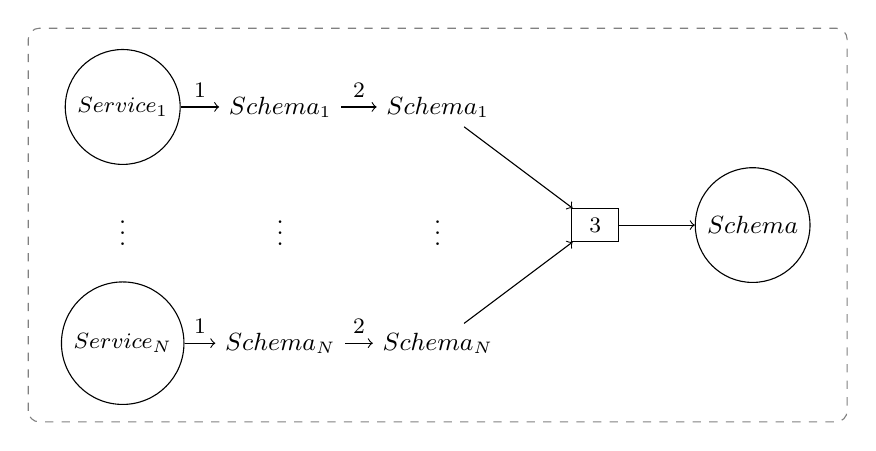
\begin{tikzpicture}[font=\small]
    \begin{pgfonlayer}{background}
      \path[rounded corners, draw=black!50, dashed] (-5.2,0) rectangle (5.2,5);
    \end{pgfonlayer}
    \node (serviceDots) at (-4,2.5) {\vdots};
    \node [circle, draw, above of=serviceDots,node distance=1.5cm,font=\footnotesize] (service1) {$Service_1$};
    \node [circle, draw, below of=serviceDots,node distance=1.5cm,font=\footnotesize] (serviceN) {$Service_N$};
    \node [right of=serviceDots,node distance=2cm] (schemaDots) {\vdots};
    \node [above of=schemaDots,node distance=1.5cm] (schema1) {$Schema_1$};
    \node [below of=schemaDots,node distance=1.5cm] (schemaN) {$Schema_N$};
    \node [right of=schemaDots,node distance=2cm] (wrappedSchemaDots) {\vdots};
    \node [above of=wrappedSchemaDots,node distance=1.5cm] (wrappedSchema1) {$Schema_1$};
    \node [below of=wrappedSchemaDots,node distance=1.5cm] (wrappedSchemaN) {$Schema_N$};
    \node [rectangle,draw,minimum width=0.6cm,font=\footnotesize,right of=wrappedSchemaDots,node distance=2cm] (deepExtendSchema) {$3$};
    \node [circle,draw,right of=deepExtendSchema,node distance=2cm] (schema) {$Schema$};
    \draw [->] (service1) -- (schema1) node [midway,above,font=\footnotesize] {$1$};
    \draw [->] (serviceN) -- (schemaN) node [midway,above,font=\footnotesize] {$1$};
    \draw [->] (schema1) -- (wrappedSchema1) node [midway,above,font=\footnotesize] {$2$};
    \draw [->] (schemaN) -- (wrappedSchemaN) node [midway,above,font=\footnotesize] {$2$};
    \draw [->] (wrappedSchema1) -- (deepExtendSchema);
    \draw [->] (wrappedSchemaN) -- (deepExtendSchema);
    \draw [->] (deepExtendSchema) -- (schema);
  \end{tikzpicture}
  \caption{Processo de criação do intermediador}
\end{figure}

\begin{figure}[H]
  \centering
  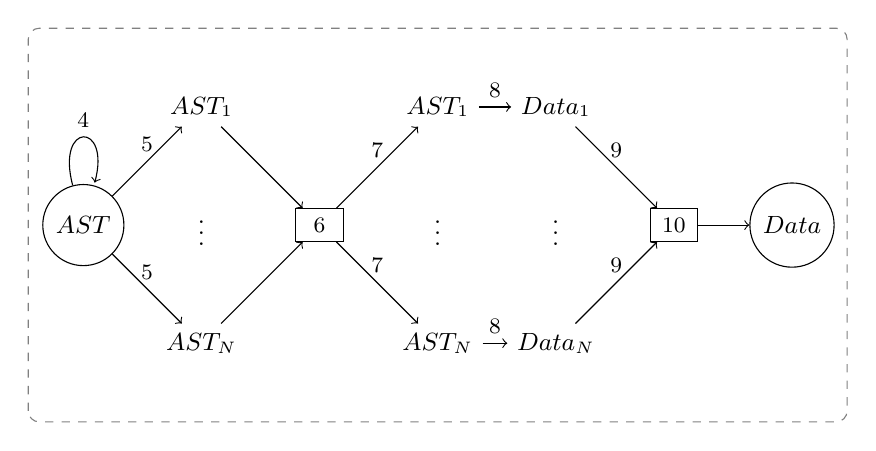
\begin{tikzpicture}[font=\small]
    \begin{pgfonlayer}{background}
      \path[rounded corners, draw=black!50, dashed] (-5.2,0) rectangle (5.2,5);
    \end{pgfonlayer}
    \node [circle, draw] (ast) at (-4.5,2.5) {$AST$};
    \node [right of=ast,node distance=1.5cm] (astTransformedDots) {\vdots};
    \node [above of=astTransformedDots,node distance=1.5cm] (astTransformed1) {$AST_1$};
    \node [below of=astTransformedDots,node distance=1.5cm] (astTransformedN) {$AST_N$};
    \node [rectangle,draw,minimum width=0.6cm,font=\footnotesize,right of=astTransformedDots,node distance=1.5cm] (reduceASTs) {$6$};
    \node [right of=reduceASTs,node distance=1.5cm] (unwrappedASTDots) {\vdots};
    \node [above of=unwrappedASTDots,node distance=1.5cm] (unwrappedAST1) {$AST_1$};
    \node [below of=unwrappedASTDots,node distance=1.5cm] (unwrappedASTN) {$AST_N$};
    \node [right of=unwrappedASTDots,node distance=1.5cm] (dataDots) {\vdots};
    \node [above of=dataDots,node distance=1.5cm] (data1) {$Data_1$};
    \node [below of=dataDots,node distance=1.5cm] (dataN) {$Data_N$};
    \node [rectangle,draw,minimum width=0.6cm,font=\footnotesize,right of=dataDots,node distance=1.5cm] (deepExtendData) {$10$};
    \node [circle, draw,right of=deepExtendData,node distance=1.5cm] (data) {$Data$};
    \draw [->,min distance=3cm,font=\footnotesize] (ast) edge[loop above] node {$4$} (ast);
    \draw [->] (ast) -- (astTransformed1) node [midway,above,font=\footnotesize] {$5$};
    \draw [->] (ast) -- (astTransformedN) node [midway,above,font=\footnotesize] {$5$};
    \draw [->] (astTransformed1) -- (reduceASTs);
    \draw [->] (astTransformedN) -- (reduceASTs);
    \draw [->] (reduceASTs) -- (unwrappedAST1) node [midway,above,font=\footnotesize] {$7$};
    \draw [->] (reduceASTs) -- (unwrappedASTN) node [midway,above,font=\footnotesize] {$7$};
    \draw [->] (unwrappedAST1) -- (data1) node [midway,above,font=\footnotesize] {$8$};
    \draw [->] (unwrappedASTN) -- (dataN) node [midway,above,font=\footnotesize] {$8$};
    \draw [->] (data1) -- (deepExtendData) node [midway,above,font=\footnotesize] {$9$};
    \draw [->] (dataN) -- (deepExtendData) node [midway,above,font=\footnotesize] {$9$};
    \draw [->] (deepExtendData) -- (data);
  \end{tikzpicture}
  \caption{Processo de consulta de dados no intermediador}
\end{figure}

O processo de criação do intermediador começa através da resolução de cada função de configuração\footnote{
  URL, metadados, adaptador e definições de envoltório.
} de serviço e construído um esquema GraphQL interno para cada um. Logo mais, é aplicado o envoltório dos campos dos esquemas e, para cada um, estende-se até gerar um esquema GraphQL unificado.

O processo de consulta de dados no intermediador começa através de uma chamada de consulta no esquema gerado. Primeiro utiliza-se o AST fornecido pela função de resolução de consulta GraphQL e converte-se para uma estrutura de maior facilidade de trabalho. Em seguida, transforma-se o AST já simplificado em ASTs específicos para o esquema de cada serviço. Durante esse processo, reduz-se as árvores através de um algoritmo de otimização de busca que analisa o conjunto como um todo. Por fim, para se poder realizar a consulta de dados correspondente em cada serviço, é desfeito o envoltório dos ASTs, realizadas as requisições e criado o envoltório e união dos dados JSON retornados. \\

\section{Proposta de Modelo}

Um novo modelo é proposto com o intuito de melhorar a comunicação cliente-servidor apresentada. Observado na figura 17, este prevê a criação de uma ferramenta no cliente para a intermediação da comunicação entre o código de busca e a API de serviços. Além disso, há a necessidade de reimplementação do código de busca para uma nova linguagem de consulta que seja interpretada pelo intermediador. Da mesma forma, soma-se a criação de um arquivo no serviço para descrição de metadados da API e outro no cliente para configuração, ambos essenciais para o funcionamento da ferramenta.

\begin{figure}[H]
  \centering
  \begin{tikzpicture}[font=\small]
    \node (client) at (-3,0) {
\includegraphics[width=1.0cm]{figuras/client}};
    \node[right of=client] (clientFetchCode) at (-2.2,0) {
\includegraphics[width=1.1cm]{figuras/code}};
    \node[below of=clientFetchCode, node distance=1.6cm] (clientLogicCode) {
\includegraphics[width=1.1cm]{figuras/code}};
    \node[above of=clientFetchCode, node distance=1.6cm] (clientConfigCode) {
\includegraphics[width=1.1cm]{figuras/code}};
    \node[rectangle,draw,right of=clientFetchCode,minimum height=1cm,minimum width=1.5cm,node distance=2.0cm] (tool) {$Tool$};
    \node[rectangle,minimum width=0.8cm, minimum height=3cm,draw,node distance=1.8cm,right of=tool,node distance=2.7cm] (api) {$API$};
    \node[right of=api, node distance=1.8cm] (data) {
\includegraphics[width=1.1cm]{figuras/code}};
    \node[below of=data,node distance=1.8cm] (server) {
\includegraphics[width=1.0cm]{figuras/server}};
    \node[above of=data, node distance=1.8cm] (metadata) {
\includegraphics[width=1.1cm]{figuras/code}};
    \node[cloud, cloud puffs=30, minimum width=11cm, minimum height=10cm, draw,style={scale=0.6}] (service) at (data) {};
    \node[below of=clientFetchCode,node distance=0.0cm] {\textless$fetch$\textgreater};
    \node[below of=clientLogicCode,node distance=0.0cm] {\textless$logic$\textgreater};
    \node[below of=clientConfigCode,node distance=0.0cm] {\textless$config$\textgreater};
    \node[below of=metadata,node distance=0.0cm] {\{$metadata$\}};
    \node[below of=data,node distance=0.0cm] {\{$data$\}};
    \node[below of=service,node distance=3.6cm] {$Service$};
    \node[below of=client,node distance=1.8cm] {\vdots};
    \node[right of=data,node distance=1.8cm] {\ldots};
    \draw[decorate,decoration={brace,raise=0.2cm,mirror}] ([yshift=6pt]clientConfigCode.north west) -- ([yshift=-12pt]clientLogicCode.south west);
    \draw [->] ([yshift=0.25cm]clientFetchCode.east) -- ([yshift=0.25cm]tool.west);
    \draw [->] (tool) -- (clientFetchCode);
    \draw [->] ([yshift=0.25cm]tool.east) -- ([yshift=0.25cm]api.west);
    \draw [->] (api) -- (tool);
    \draw [->,dashed] (clientConfigCode) -| ([xshift=-0.25cm]tool.north);
    \draw [->,dashed] (metadata) -| ([xshift=0.25cm]tool.north);
  \end{tikzpicture}
  \caption{Modelo proposto para evitar contrato de comunicação}
\end{figure}

A proposta de eliminação de contrato visa também automatizar o acesso de clientes em APIs. Através da implementação de algoritmos na ferramenta, escolhe-se o caminho de acesso de melhor custo-benefício em relação aos serviços disponíveis para o cliente. O modelo proporciona, além disso, um ambiente escalável para consulta de dados através da composição de serviços, visto na figura 18.

\begin{figure}[H]
  \centering
  \begin{tikzpicture}[font=\small]
    \node (client1) at (-2,0) {
\includegraphics[width=1.0cm]{figuras/client}};
    \node (client2) at (2,0) {
\includegraphics[width=1.0cm]{figuras/client}};
    \node[rectangle,draw,minimum height=1cm,minimum width=1.5cm,below of=client2,node distance=2.3cm] (tool) {$Tool$};
    \node[cloud, cloud puffs=16, draw] (service1) at (-3,-6) {$Service_1$};
    \node (serviceDots) at (0,-6) {\ldots};
    \node[cloud, cloud puffs=16,minimum height=1cm, draw] (serviceN) at (3,-6) {$Service_N$};
    \draw [->] (client1) -- (service1) node [midway,above,font=\footnotesize] {$request$};
    \draw [->] (client1) -- (serviceN) node [midway,above,font=\footnotesize] {$request$};
    \draw [->] (client2) -- (tool) node [midway,above,font=\footnotesize] {$query$};
    \draw [->] (tool) -- (service1) node [midway,above,font=\footnotesize] {$request$};
    \draw [->] (tool) -- (serviceN) node [midway,above,font=\footnotesize] {$request$};
  \end{tikzpicture}
  \caption{Composição de serviços através da ferramenta}
\end{figure}

\section{Especificação da Ferramenta}

Visando a aceitação da ferramenta prevista pelo modelo em ambientes de desenvolvimento de clientes, foi preciso pensar em uma especificação que apresentasse uma interface de baixa curva de aprendizagem, um fluxo de execução replicável e agnóstico à plataforma, além do baixo impacto na base de código de clientes. Por conseguinte, a ferramenta proposta foi desenvolvida pensando na reutilização de tecnologias promissoras ou bem consolidadas no mercado de desenvolvimento.

Com a sucessão de estudos, a escolha foi em utilizar a tecnologia GraphQL como principal biblioteca para ajudar com intermediação da comunicação do modelo proposto. Ao invés da tecnologia Falcor (apontada durante o estudo), GraphQL foi o único que apresentou uma solução robusta que permitisse o acesso de APIs Web por clientes através de consultas em seu código de busca. Da mesma forma, buscou-se trabalhar com formatos abertos de descrição de metadados de APIs, como por exemplo o JSON Hyper-Schema. Através de adaptadores, a ferramenta permite acelerar a integração de serviços que já oferecem metadados em formatos suportados.

A seguir, é realizada a análise dos dois fluxos de execução descritos na especificação da ferramenta. O primeiro, ilustrado na figura 20, é o processo de criação do intermediador, que recebe de entrada funções de configuração de serviços e retorna um esquema GraphQL. O segundo, mostrado na figura 21, é o processo de consulta de dados no intermediador, que recebe de entrada consultas escritas na sintaxe da linguagem GraphQL e, após chamadas às APIs, retorna estruturas de dados JSON.

\begin{figure}[H]
  \centering
  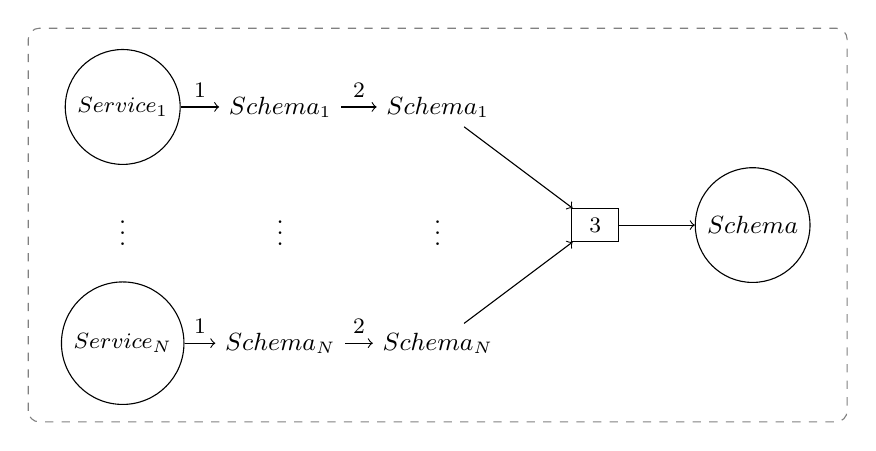
\begin{tikzpicture}[font=\small]
    \begin{pgfonlayer}{background}
      \path[rounded corners, draw=black!50, dashed] (-5.2,0) rectangle (5.2,5);
    \end{pgfonlayer}
    \node (serviceDots) at (-4,2.5) {\vdots};
    \node [circle, draw, above of=serviceDots,node distance=1.5cm,font=\footnotesize] (service1) {$Service_1$};
    \node [circle, draw, below of=serviceDots,node distance=1.5cm,font=\footnotesize] (serviceN) {$Service_N$};
    \node [right of=serviceDots,node distance=2cm] (schemaDots) {\vdots};
    \node [above of=schemaDots,node distance=1.5cm] (schema1) {$Schema_1$};
    \node [below of=schemaDots,node distance=1.5cm] (schemaN) {$Schema_N$};
    \node [right of=schemaDots,node distance=2cm] (wrappedSchemaDots) {\vdots};
    \node [above of=wrappedSchemaDots,node distance=1.5cm] (wrappedSchema1) {$Schema_1$};
    \node [below of=wrappedSchemaDots,node distance=1.5cm] (wrappedSchemaN) {$Schema_N$};
    \node [rectangle,draw,minimum width=0.6cm,font=\footnotesize,right of=wrappedSchemaDots,node distance=2cm] (deepExtendSchema) {$3$};
    \node [circle,draw,right of=deepExtendSchema,node distance=2cm] (schema) {$Schema$};
    \draw [->] (service1) -- (schema1) node [midway,above,font=\footnotesize] {$1$};
    \draw [->] (serviceN) -- (schemaN) node [midway,above,font=\footnotesize] {$1$};
    \draw [->] (schema1) -- (wrappedSchema1) node [midway,above,font=\footnotesize] {$2$};
    \draw [->] (schemaN) -- (wrappedSchemaN) node [midway,above,font=\footnotesize] {$2$};
    \draw [->] (wrappedSchema1) -- (deepExtendSchema);
    \draw [->] (wrappedSchemaN) -- (deepExtendSchema);
    \draw [->] (deepExtendSchema) -- (schema);
  \end{tikzpicture}
  \caption{Processo de criação do intermediador}
\end{figure}

\begin{figure}[H]
  \centering
  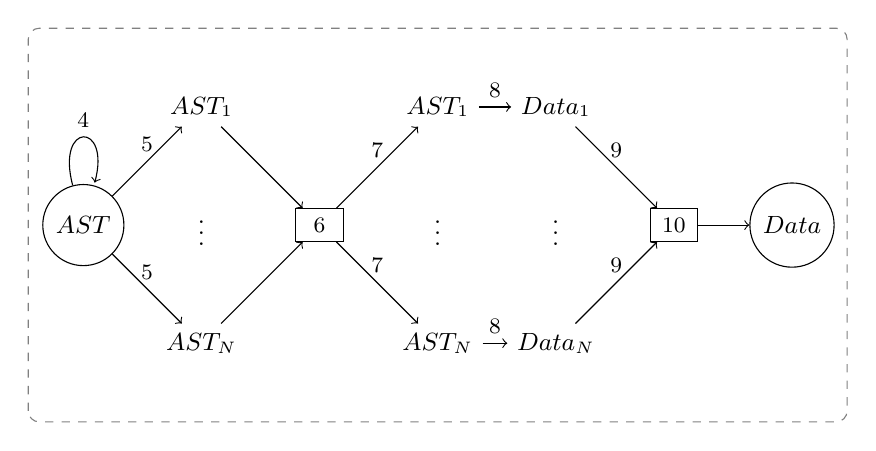
\begin{tikzpicture}[font=\small]
    \begin{pgfonlayer}{background}
      \path[rounded corners, draw=black!50, dashed] (-5.2,0) rectangle (5.2,5);
    \end{pgfonlayer}
    \node [circle, draw] (ast) at (-4.5,2.5) {$AST$};
    \node [right of=ast,node distance=1.5cm] (astTransformedDots) {\vdots};
    \node [above of=astTransformedDots,node distance=1.5cm] (astTransformed1) {$AST_1$};
    \node [below of=astTransformedDots,node distance=1.5cm] (astTransformedN) {$AST_N$};
    \node [rectangle,draw,minimum width=0.6cm,font=\footnotesize,right of=astTransformedDots,node distance=1.5cm] (reduceASTs) {$6$};
    \node [right of=reduceASTs,node distance=1.5cm] (unwrappedASTDots) {\vdots};
    \node [above of=unwrappedASTDots,node distance=1.5cm] (unwrappedAST1) {$AST_1$};
    \node [below of=unwrappedASTDots,node distance=1.5cm] (unwrappedASTN) {$AST_N$};
    \node [right of=unwrappedASTDots,node distance=1.5cm] (dataDots) {\vdots};
    \node [above of=dataDots,node distance=1.5cm] (data1) {$Data_1$};
    \node [below of=dataDots,node distance=1.5cm] (dataN) {$Data_N$};
    \node [rectangle,draw,minimum width=0.6cm,font=\footnotesize,right of=dataDots,node distance=1.5cm] (deepExtendData) {$10$};
    \node [circle, draw,right of=deepExtendData,node distance=1.5cm] (data) {$Data$};
    \draw [->,min distance=3cm,font=\footnotesize] (ast) edge[loop above] node {$4$} (ast);
    \draw [->] (ast) -- (astTransformed1) node [midway,above,font=\footnotesize] {$5$};
    \draw [->] (ast) -- (astTransformedN) node [midway,above,font=\footnotesize] {$5$};
    \draw [->] (astTransformed1) -- (reduceASTs);
    \draw [->] (astTransformedN) -- (reduceASTs);
    \draw [->] (reduceASTs) -- (unwrappedAST1) node [midway,above,font=\footnotesize] {$7$};
    \draw [->] (reduceASTs) -- (unwrappedASTN) node [midway,above,font=\footnotesize] {$7$};
    \draw [->] (unwrappedAST1) -- (data1) node [midway,above,font=\footnotesize] {$8$};
    \draw [->] (unwrappedASTN) -- (dataN) node [midway,above,font=\footnotesize] {$8$};
    \draw [->] (data1) -- (deepExtendData) node [midway,above,font=\footnotesize] {$9$};
    \draw [->] (dataN) -- (deepExtendData) node [midway,above,font=\footnotesize] {$9$};
    \draw [->] (deepExtendData) -- (data);
  \end{tikzpicture}
  \caption{Processo de consulta de dados no intermediador}
\end{figure}

Os passos enumerados nas figuras 20 e 21 são descritos a seguir:

\begin{enumerate}
  \item Constrói um esquema GraphQL para o serviço através de seus metadados. Este processo pode ser sobrescrito por adaptadores.
  \item Envolve os campos do esquema GraphQL gerado para o serviço visando facilitar a consulta e, depois, unificar com outros esquemas de maneira correta.
  \item Realiza a união dos esquemas GraphQL gerados para cada serviço. Cria um esquema unificado para que a ferramenta possa interpretar consultas de diversos serviços em uma única operação.
  \item Simplifica o AST gerado pela consulta no esquema unificado para facilitar o trabalho na resolução de fragmentos GraphQL.
  \item Transforma o AST principal da consulta em um AST especifico para cada esquema de serviço. Dessa forma, separa os dados que cada serviço consegue disponibilizar para o cliente. Este processo pode ser sobrescrito por adaptadores.
  \item Analisa os ASTs gerados para cada serviço na etapa de transformação e, a partir de heurísticas, reduz os campos dos ASTs para otimizar consultas. A heurística envolve o número de requisições necessárias para número de dados retornados e requisições para obtê-los.
  \item Desfaz o envoltório do AST para poder realizar a requisição correta na consulta dos dados do serviço.
  \item Busca os dados a partir do AST, onde interpreta os metadados do serviço e realiza requisições para a API do serviço. Este processo pode ser sobrescrito por adaptadores.
  \item Recria o envoltório dos dados retornados para que o esquema GraphQL entenda e consiga unificar com outros dados de maneira correta.
  \item Unifica os dados retornados pelas APIs de cada serviço, nas quais foram feitas as requisições.
\end{enumerate}

Em resumo, o processo de criação do intermediador começa através da resolução das funções de configuração de serviços (URL, metadados, adaptador e definições de envoltório) para construir um esquema GraphQL de cada um. Na sequência, é aplicado o envoltório dos campos dos esquemas, estendendo-se até gerar um esquema GraphQL unificado.

Com relação ao processo de consulta de dados no intermediador, este começa através de uma chamada de consulta no esquema gerado. Primeiramente utiliza-se o AST fornecido pela função de resolução de consulta GraphQL e converte-se para uma estrutura de maior facilidade de trabalho. Em seguida, transforma-se o AST já simplificado em ASTs específicos para o esquema de cada serviço. Durante esse processo, reduz-se as árvores através de um algoritmo de otimização de busca que analisa o conjunto como um todo. Por fim, para se poder realizar a consulta de dados correspondente em cada serviço, é desfeito o envoltório dos ASTs, são realizadas as requisições, é criado o envoltório e é feita a união dos dados JSON retornados.

\section{Implementação da Ferramenta}

A fim de aplicar a especificação da ferramenta abordada no planejamento de projeto, foi proposta a implementação de onze funções, divididas em três categorias, para o uso de clientes na plataforma Web. Cada uma dessas funções levantadas resolve um problema com o intuito de chegar ao objetivo de representar os dois fluxos de execução.

Dentro do conjunto de funções, quatro delas são responsáveis por criar o intermediador; três funções analisam as consultas através do formato AST; e as outras quatro transformam as consultas em requisições para API de serviços. Somente quatro são públicas e expostas para o cliente, sendo uma delas (composeSchema) a principal para criação do esquema de consulta, e as outras três (buildSchema, transformAST, fetchData) para serem sobrescritas por adaptadores.

A seguir, são descritas brevemente essas três categorias de funções, ao lado de seu objetivo e a assinatura JavaScript de cada função em Flow\footnote{
  Verificador de tipo estático para JavaScript.
}. \\

\textbf{Criação do esquema} \\

Consiste de quatro funções e seu principal objetivo é compor, de forma assíncrona, um esquema GraphQL unificado a partir das funcões de configuração de cada serviço.

\begin{figure}[H]
  \centering
  \begin{minted}[frame=single,framesep=10pt,fontsize=\footnotesize]{text}
  function composeSchema(
    services: [Service]
  ): Promise<GraphQLSchema>

  function buildSchema(
    metadata: JSON
  ): Promise<GraphQLSchema>

  function wrapSchema(
    schema: GraphQLSchema,
    wrapper: JSON
  ): Promise<GraphQLSchema>

  function deepExtendSchema(
    schemas: [GraphQLSchema]
  ): Promise<GraphQLSchema>
  \end{minted}
  \caption{Assinatura JS das funções para criação do esquema}
\end{figure}

\textbf{Análise de consulta} \\

É constituído de três funções que buscam analisar consultas GraphQL executadas no esquema gerado em formato AST. A análise descreve algoritmos que simplificam, transformam e reduzem o AST principal da consulta, quebrando-o em ASTs específicos para cada serviço.

\begin{figure}[H]
  \centering
  \begin{minted}[frame=single,framesep=10pt,fontsize=\footnotesize]{text}
  function simplifyAST(
    value: AST,
    info: JSON
  ): SimplifiedAST

  function transformAST(
    metadata: JSON,
    schema: GraphQLSchema,
    ast: SimplifiedAST
  ): SimplifiedAST

  function reduceASTs(
    rootAST: SimplifiedAST,
    asts: [SimplifiedAST]
  ): [SimplifiedAST]
  \end{minted}
  \caption{Assinatura JS das funções para análise de consulta}
\end{figure}

\textbf{Consulta de dados} \\

Consiste as quatro últimas funções responsáveis por converter os ASTs de cada serviço e realizar as respectivas requisições para consulta de dados sobre APIs.

\begin{figure}[H]
  \centering
  \begin{minted}[frame=single,framesep=10pt,fontsize=\footnotesize]{text}
  function unwrapAST(
    ast: SimplifiedAST,
    schema: GraphQLSchema,
    wrapper: JSON
  ): SimplifiedAST

  function fetchData(
    metadata: JSON,
    ast: SimplifiedAST,
    url: String
  ): Promise<JSON>

  function wrapData(
    data: JSON,
    schema: GraphQLSchema,
    wrapper: JSON
  ): JSON

  function deepExtendData(
    data: [JSON]
  ): JSON
  \end{minted}
  \caption{Assinatura JS das funções para consulta de dados}
\end{figure}


\chapter{Validação}

Com o objetivo de validar o modelo proposto, é realizada uma pesquisa comparativa com foco no impacto em relação ao uso da ferramenta implementada e mudanças no fluxo de dados sobre APIs Web. Para isso, é desenvolvido um ambiente de validação onde dois clientes, um com a ferramenta e o outro não, realizam três consultas de dados sobre a API de um serviço REST. Por fim, é aplicada uma série de quatro mudanças no fluxo de dados da API e coletados os dados para análise do impacto causado no código de busca desses clientes. \\

\textbf{Escopo de serviço} \\

Foi escolhido trabalhar com um escopo de serviço conhecido como SWAPI (\textit{Starwars API}), bastante utilizado para análise de implementações de tecnologias e estilos de arquitetura em linguagens de programação. Nele, são descritos seis entidades (Pessoa, Filme, Espaçonave, Veículo, Espécie, Planeta) e seus respectivos relacionamentos. Dentro do escopo de serviço, é implementado uma API REST que expõe consultas dessas entidades em formato de representação JSON através de URIs, visto na tabela 6. Nota-se que as representações possuem apenas um nível de expansão, ou seja, para acesso dos relacionamentos é preciso consultar a API através de links descritos pela estrutura de retorno (HATEOAS).

\begin{table}[H]
  \centering
  \begin{tabular}{|l|c|}
    \hline
    URI & Descrição \\
    \hline
    /people & Busca lista de pessoas \\
    \hline
    /people/:id & Busca pessoa pelo id \\
    \hline
    /films & Busca lista de filmes \\
    \hline
    /films/:id & Busca filme pelo id \\
    \hline
    /starships & Busca lista de espaçonaves \\
    \hline
    /starships/:id & Busca espaçonave pelo id \\
    \hline
    /vehicles & Busca lista de veículos \\
    \hline
    /vehicles/:id & Busca veículo pelo id \\
    \hline
    /species & Busca lista de espécies \\
    \hline
    /species/:id & Busca espécie pelo id \\
    \hline
    /planets & Busca lista de planetas \\
    \hline
    /planets/:id & Busca planeta pelo id \\
    \hline
  \end{tabular}
  \caption{Pontos de acesso (GET) SWAPI}
\end{table}

\textbf{Perguntas e respostas esperadas} \\

Com o propósito de explorar cada ponto de acesso para busca de dados na SWAPI, foram determinadas três perguntas de média complexidade, onde fossem envolvidos ao menos três das entidades do escopo. Para cada pergunta existe apenas uma resposta certa, onde sua lógica é baseada em campos das estruturas de dados de retorno.

\begin{enumerate}
\item[\textbf{Q1.}] Qual o nome do filme no qual aparecem mais personagens oriundos de um planeta deserto? \textbf{R:} "Revenge of the Sith"
\item[\textbf{Q2.}] Qual o nome da espécie predominante entre os habitantes do planeta "Tatooine"? \textbf{R:} "Droid"
\item[\textbf{Q3.}] Qual o nome do personagem que mais pilota espaçonaves e veículos durante o filme "A New Hope"? \textbf{R:} "Chewbacca"
\end{enumerate}

No intuito de atingir as respostas esperadas, a tabela 7 descreve o fluxo de dados necessário de cada pergunta para a busca de dados por clientes.

\begin{table}[H]
  \centering
  \begin{tabular}{|c|c|c|}
    \hline
    Pergunta & Fluxo de Dados & Número de requisições \\
    \hline
    Q1 & \begin{minipage}[t]{0.3\textwidth}
      \begin{itemize}
        \item[\textbf{GET}] /api/films
        \item[\textbf{GET}] /api/people/:id
        \item[\textbf{GET}] /api/planet/:id
      \end{itemize}
    \end{minipage} & \begin{minipage}[t]{0.5\textwidth}
      \begin{itemize}
        \item[\textbf{x1}] films
        \item[\textbf{x162}] films.characters
        \item[\textbf{x162}] films.characters.homeworld
      \end{itemize}
    \end{minipage} \\
    \hline
    Q2 & \begin{minipage}[t]{0.3\textwidth}
      \begin{itemize}
        \item[\textbf{GET}] /api/planets/1
        \item[\textbf{GET}] /api/people/:id
        \item[\textbf{GET}] /api/species/:id
      \end{itemize}
    \end{minipage} & \begin{minipage}[t]{0.5\textwidth}
      \begin{itemize}
        \item[\textbf{x1}] planet
        \item[\textbf{x10}] planet.residents
        \item[\textbf{x2}] planet.residents.species
      \end{itemize}
    \end{minipage} \\
    \hline
    Q3 & \begin{minipage}[t]{0.3\textwidth}
      \begin{itemize}
        \item[\textbf{GET}] /api/films/1
        \item[\textbf{GET}] /api/starships/:id
        \item[\textbf{GET}] /api/people/:id
        \item[\textbf{GET}] /api/vehicles/:id
        \item[\textbf{GET}] /api/people/:id
      \end{itemize}
    \end{minipage} & \begin{minipage}[t]{0.5\textwidth}
      \begin{itemize}
        \item[\textbf{x1}] film
        \item[\textbf{x8}] film.starships
        \item[\textbf{x9}] film.starships.pilots
        \item[\textbf{x4}] film.vehicles
        \item[\textbf{x0}] film.vehicles.pilots
      \end{itemize}
    \end{minipage} \\
    \hline
  \end{tabular}
  \caption{Fluxo de dados para responder as perguntas}
\end{table}

\textbf{Consultas e metadados} \\

Para permitir a comunicação entre o cliente que faz o uso da ferramenta com a SWAPI, foi preciso implementar três consultas GraphQL (uma para cada pergunta), além de descrever os metadados da API REST. Nas consultas da figura 26, foram realizadas apenas a busca de dados necessários para o funcionamento da lógica de resposta. Enquanto aos metadados da figura 27, foram descritos apenas as URIs utilizadas no formato JSON Hyper-Schema, junto com implementação de um adaptador para a ferramenta que consiga interpretar este formato.

\begin{figure}[H]
  \centering
  \begin{minted}[frame=single,framesep=10pt,fontsize=\footnotesize]{text}
      query q1 {
        allFilms {
          title
          characters {
            homeworld {
              climate
            }
          }
        }
      }

      query q2 {
        planet(planetID: 1) {
          residents {
            species {
              name
            }
          }
        }
      }

      query q3 {
        film(filmID: 1) {
          starships {
            pilots {
              name
            }
          }
          vehicles {
            pilots {
              name
            }
          }
        }
      }
  \end{minted}
  \caption{Consultas GraphQL para as perguntas}
\end{figure}

\begin{figure}[H]
  \centering
  \begin{minted}[frame=single,framesep=10pt,fontsize=\footnotesize]{text}
    {
      "$schema": "http://json-schema.org/draft-04/hyper-schema#",
      "title": "swapi",
      "type": "object",
      "definitions": {
        "allFilms": { ... },
        "film": { ... },
        "people": { ... },
        "planet": { ... },
        "species": { ... },
        "starship": { ... },
        "vehicle": { ... }
      },
      "properties": {
        "allFilms": { "$ref": "#/definitions/allFilms" },
        "film": { "$ref": "#/definitions/film" },
        "people": { "$ref": "#/definitions/people" },
        "planet": { "$ref": "#/definitions/planet" },
        "species": { "$ref": "#/definitions/species" },
        "starship": { "$ref": "#/definitions/starship" }
      },
      "links": [{
        "rel": "allFilms",
        "href": "/films",
        "targetSchema": {
          "$ref": "#/definitions/allFilms"
        }
      }, {
        "rel": "film",
        "href": "/films/{filmID}",
        "schema": { ... },
        "targetSchema": {
          "$ref": "#/definitions/film"
        }
      }, {
        "rel": "planet",
        "href": "/planets/{planetID}",
        "schema": { ... },
        "targetSchema": {
          "$ref": "#/definitions/planet"
        }
      }]
    }
  \end{minted}
  \caption{JSON Hyper-Schema para SWAPI}
\end{figure}

\textbf{Mudanças no fluxo de dados} \\

Para avaliar o impacto no código em ambos clientes, é proposto quatro tipos de mudanças na API não acumulativas que afetam o fluxo de dados. Cada uma busca testar a capacidade da ferramenta em se adaptar e realizar a comunicação mesmo após a alteração no fluxo. Nota-se que, para cada mudança na API do serviço, é preciso a atualização de seus metadados para a correta operação da ferramenta. A tabela 8 descreve o changelog das mudanças realizadas.

\begin{table}[H]
  \centering
  \begin{tabular}{|c|c|c|}
    \hline
    Mudança & Descrição & Changelog \\
    \hline
    C1 & \begin{minipage}[t]{0.3\textwidth}
      Mudança no endereço de ponto de acesso.
    \end{minipage} & \begin{minipage}[t]{0.5\textwidth}
      \begin{itemize}
        \item Renomeação da URI /films para /movies.
        \item Renomeação da URI /films/:id para /movies/:id
      \end{itemize}
    \end{minipage} \\
    \hline
    C2 & \begin{minipage}[t]{0.3\textwidth}
      Mudança no nível de estrutura de resposta.
    \end{minipage} & \begin{minipage}[t]{0.5\textwidth}
      \begin{itemize}
        \item Expansão do campo pilots da URI /starships/:id
        \item Expansão do campo pilots da URI /vehicles/:id
      \end{itemize}
    \end{minipage} \\
    \hline
    C3 & \begin{minipage}[t]{0.3\textwidth}
      Adição de ponto de acesso otimizado.
    \end{minipage} & \begin{minipage}[t]{0.5\textwidth}
      \begin{itemize}
        \item[\textbf{+}] Adição da URI /tatooine.
        \item[\textbf{+}] Adição da URI /films/:id/characters.
      \end{itemize}
    \end{minipage} \\
    \hline
    C4 & \begin{minipage}[t]{0.3\textwidth}
      Remoção de ponto de acesso deprecado.
    \end{minipage} & \begin{minipage}[t]{0.5\textwidth}
      \begin{itemize}
        \item[\textbf{+}] Adição da URI /people/:id/homeworld.
        \item[\textbf{$-$}] Remoção da URI /planet/:id.
      \end{itemize}
    \end{minipage} \\
    \hline
  \end{tabular}
  \caption{Changelog do novo fluxo de dado para cada mudança}
\end{table}

\textbf{Variáveis} \\

São descritas cinco variáveis para análise dos quatro testes de validação em cada um dos clientes. Todas são quantitativas e coletadas no cliente após cada processo de mudança da API. Dessa maneira, totalizam um número de 40 dados normalizados possíveis para análise no final da execução nos dois clientes.

\begin{table}[H]
  \centering
  \begin{tabular}{|c|c|c|}
    \hline
    Variável & Unidade & Tipo \\
    \hline
    Porcentagem de acerto & \% & Quantitativa \\
    \hline
    Tamanho de resposta & kb & Quantitativa \\
    \hline
    Número de requisições & inteiro & Quantitativa \\
    \hline
    Tempo de busca de metadados & ms & Quantitativa \\
    \hline
    Tempo de processamento & ms & Quantitativa \\
    \hline
  \end{tabular}
  \caption{Variáveis de coleta e análise}
\end{table}

\section{Resultados}

Os resultados obtidos nos testes de validação apresentam a média dos valores coletados após diversas execuções dos quatro testes de mudança de forma sequencial em uma máquina virtual. Tanto o serviço SWAPI como os clientes JavaScript foram executados no mesmo ambiente computacional, porém com conexão local de latência 10mb/s para simulação de um ambiente distribuído. Para a variável de processamento, foram utilizados valores que pudessem representar um dispositivo computacional de médio porte. (1 CPU de 2.4 GHz e 4gb de RAM)

Inicialmente, observa-se na figura 27 que o cliente 1 (sem o uso da ferramenta) não apresenta um bom índice de acerto das respostas. Dentre as quatro mudanças, obteve apenas 58\% de acerto, sendo a C3 a única mudança em que conseguiu responder certo todas pois não houve mudança nas URIs que estava utilizando. Um resultado esperado, significando que houve quebra de contrato e impacto negativo ao código de busca.

Em contrapartida, o cliente 2 (com o uso da ferramenta) apresenta um resultado no índice de acerto da figura 28 36.61\% superior ao cliente 1. Com um total de 91,5\% de acerto, apenas não completou com 100\% de acerto pois a mudança C4 não permitiu que fosse possível acessar todos os dados necessários para a responder da pergunta Q2. Isso representa que a ferramenta foi capaz, através do intermediador, de evitar a criação de contrato e causar impacto negativo ao código de busca.

Nota-se que ambos os clientes não apresentaram erros na resposta, ao invés acabam não respondendo pois ocorre exceções durante o código de busca ou lógica devido ao impacto das mudanças no fluxo de dados.

\begin{figure}[H]
  \centering
  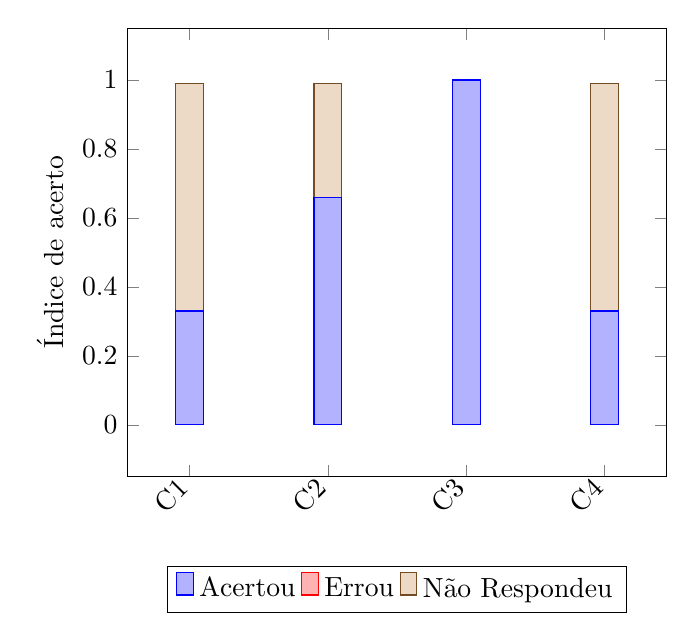
\begin{tikzpicture}
  \begin{axis}[
      ybar stacked,
      ymax=1,
      ymin=0,
      enlargelimits=0.15,
      legend style={at={(0.5,-0.20)},
        anchor=north,legend columns=-1},
      ylabel={Índice de acerto},
      symbolic x coords={C1, C2, C3, C4,
          C5, C6, C7},
      xtick=data,
      x tick label style={rotate=45,anchor=east},
      ]
  \addplot+[ybar] plot coordinates {(C1,0.33) (C2,0.66)
    (C3,1) (C4,0.33)};
  \addplot+[ybar] plot coordinates {(C1,0) (C2,0)
    (C3,0) (C4,0)};
  \addplot+[ybar] plot coordinates {(C1,0.66) (C2,0.33)
    (C3,0) (C4,0.66)};
  \legend{Acertou, Errou, Não Respondeu}
  \end{axis}
  \end{tikzpicture}
  \caption{Índice de acerto sem o uso da ferramenta}
\end{figure}

\begin{figure}[H]
  \centering
  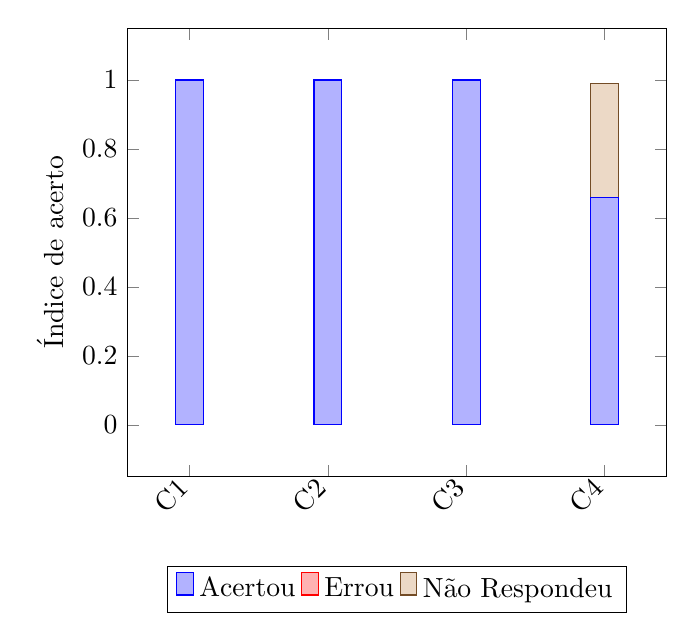
\begin{tikzpicture}
  \begin{axis}[
      ybar stacked,
      ymax=1,
      ymin=0,
      enlargelimits=0.15,
      legend style={at={(0.5,-0.20)},
        anchor=north,legend columns=-1},
      ylabel={Índice de acerto},
      symbolic x coords={C1, C2, C3, C4,
          C5, C6, C7},
      xtick=data,
      x tick label style={rotate=45,anchor=east},
      ]
  \addplot+[ybar] plot coordinates {(C1,1) (C2,1)
    (C3,1) (C4,0.66)};
  \addplot+[ybar] plot coordinates {(C1,0) (C2,0)
    (C3,0) (C4,0)};
  \addplot+[ybar] plot coordinates {(C1,0) (C2,0)
    (C3,0) (C4,0.33)};
  \legend{Acertou, Errou, Não Respondeu}
  \end{axis}
  \end{tikzpicture}
  \caption{Índice de acerto com o uso da ferramenta}
\end{figure}

Ao analisar a mudança C3 isoladamente, onde ambos conseguem responder com 100\% de acerto, percebe-se na figura 29 e 30 que o cliente 2 consegue realizar uma busca mais performática (menor número de requisição e tamanho de dados) que o cliente 1. Isso porque, após a mudança e sem alterar o código de busca de dados, a ferramenta consegue remapear as requisições geradas pelas consultas GraphQL graças ao algoritmo de implementação na automação das chamadas em URIs.

Outro ponto importante é que, após a mudança C3 e atualização dos metadados no cliente, o algoritmo da ferramenta percebe que há a possibilidade de realizar menos requisições em busca dos dados para responder as perguntas. O que resulta em uma redução de aproximadamente 54\% dos acessos entre o cliente 1 e cliente 2.

\begin{figure}[H]
  \centering
  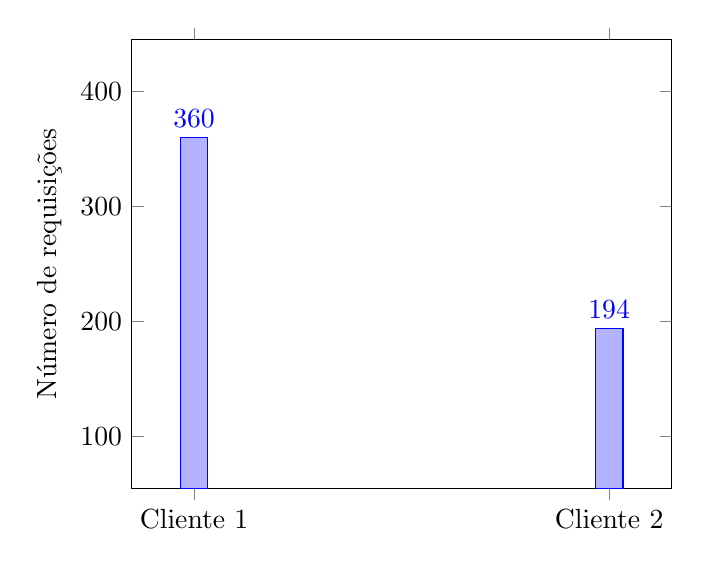
\begin{tikzpicture}
  \begin{axis}[
      ybar,
      ymax=400,
      ymin=100,
      enlargelimits=0.15,
      ylabel={Número de requisições},
      symbolic x coords={Cliente 1,Cliente 2},
      xtick=data,
      nodes near coords,
      nodes near coords align={vertical},
      ]
  \addplot coordinates {(Cliente 1,360) (Cliente 2,194)};
  \end{axis}
  \end{tikzpicture}
  \caption{Comparação no número de requisições C3}
\end{figure}

\begin{figure}[H]
  \centering
  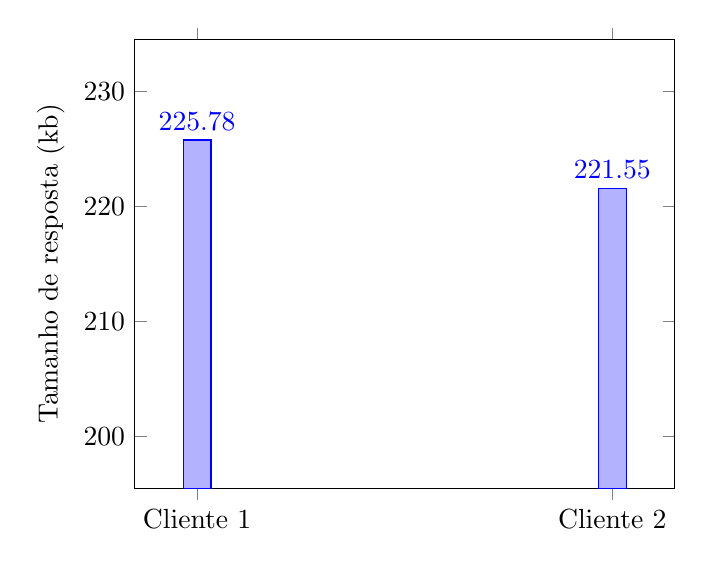
\begin{tikzpicture}
  \begin{axis}[
      ybar,
      ymax=230,
      ymin=200,
      enlargelimits=0.15,
      ylabel={Tamanho de resposta (kb)},
      symbolic x coords={Cliente 1,Cliente 2},
      xtick=data,
      nodes near coords,
      nodes near coords align={vertical},
      ]
  \addplot coordinates {(Cliente 1,225.777) (Cliente 2,221.547)};
  \end{axis}
  \end{tikzpicture}
  \caption{Comparação no tamanho de resposta C3}
\end{figure}

Apesar dos ganhos de performance e desenvolvimento através do uso da ferramenta vistos anteriormente, percebe-se na figura 31 um outro cenário em que indica o lado negativo do seu uso causado pelo tempo de \textit{overhead}\footnote{
  Processamento em excesso
}. Em média, a ferramenta atrasou em 1.7 segundos a execução na consulta de dados do cliente, sendo o tempo de busca de metadados responsável por somar mais da metade deste atraso inicial.

Contudo, é importante levar em conta que este tempo de \textit{overhead} é um impasse da ferramenta, mas também relativo ao tempo de vida do cliente que está sendo executado. Por exemplo, em clientes com tempo de vida curto ou que dependem de carregamento rápido, a ferramenta pode não ser a solução ideal. Nos demais casos, é visível os benefícios que seu uso pode trazer.

\begin{figure}[H]
  \centering
  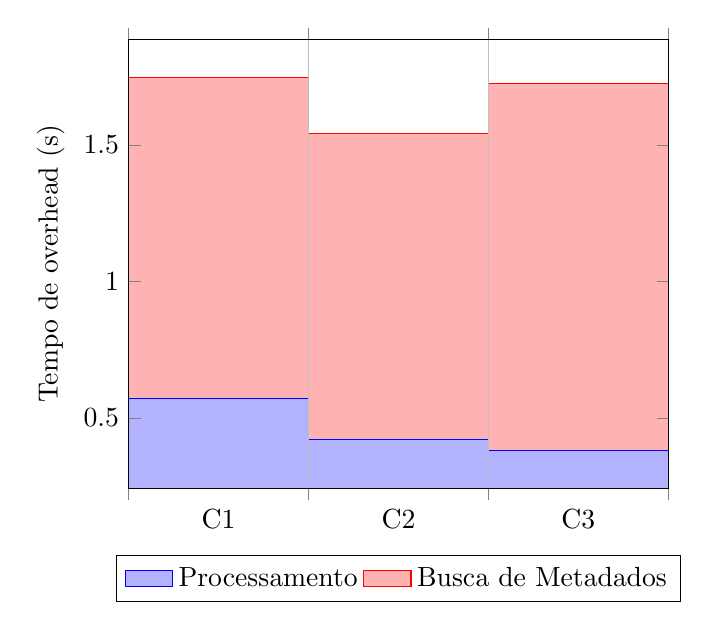
\begin{tikzpicture}
	\begin{axis}[
        ybar interval,
        ylabel={Tempo de overhead (s)},
        legend style={at={(0.5,-0.15)},
        anchor=north,legend columns=-1},
        const plot,
		stack plots=y,
		area style,
        symbolic x coords={C1,C2,C3,C4},
		enlarge x limits=false]
	\addplot coordinates
		{(C1,0.57) (C2,0.42) (C3,0.38) (C4,0.48)}
		\closedcycle;
	\addplot coordinates
		{(C1,1.178) (C2,1.123) (C3,1.343) (C4,1.185)}
		\closedcycle;
    \legend{Processamento,Busca de Metadados}
	\end{axis}
  \end{tikzpicture}
  \caption{Overhead da ferramenta}
\end{figure}


\chapter{Conclusão}

Tornam-se evidentes, através deste trabalho, as dificuldades de serviços em realizar mudanças na especificação de APIs uma vez que estas já possuem clientes fazendo o seu acesso. Além disso, nota-se que é possível explorar novos modelos de comunicação a fim de manter a eficiência da comunicação cliente-servidor evitando versionamento.

O esforço dedicado neste trabalho em explorar esta área culminou no desenvolvimento de um novo modelo de comunicação. Buscou-se eliminar a preocupação de clientes em estar continuamente atualizando seu código de busca a cada mudança na API e direcionar desenvolvedores de clientes à implementação de códigos de busca independentes de especificação de API.

Apesar das vantagens do modelo, existe um investimento a mais com a integração da ferramenta para que clientes e serviços possam usufruir os benefícios demonstrados nos resultados dos testes de validação. Felizmente, serviços que disponibilizam descrições de metadados da sua API apresentam uma menor barreira de entrada e já podem ser consultados utilizando a ferramenta.

Por fim, uma das principais contribuições deste trabalho é estampar os benefícios da automação na execução de consultas de dados e composição de serviços que o modelo e a ferramenta podem proporcionar. Basta que os desenvolvedores de clientes se preocupem em escrever um código de busca através de linguagens de consulta como o GraphQL e dos serviços em disponibilizarem uma completa descrição dos metadados de APIs.

\section[Trabalhos Futuros]{Trabalhos Futuros}

\begin{itemize}
  \item Realização de testes de validação para a composição de serviços.
  \item Criação de novos adaptadores da ferramenta para formatos de descrição de APIs. (OpenAPI, RAML, API Blueprint)
  \item Implementação da especificação da ferramenta em outras plataformas de desenvolvimento. (Mobile, Desktop, etc)
  \item Aprimoramento do algoritmo de análise de consultas.
\end{itemize}

Identificamos as seguintes possibilidades de continuidade e evolução deste trabalho: 

\begin{itemize}
\item Realização de testes de validação para a composição de serviços.
\item Criação de novos adaptadores da ferramenta para formatos de descrição de APIs. (OpenAPI, RAML, API Blueprint)
\item Implementação da especificação da ferramenta em outras plataformas de desenvolvimento. (Mobile, Desktop, etc)
\item Aprimoramento do algoritmo de análise de consultas.
\end{itemize}


\bibliography{bibliografia/index}
\end{document}
